\documentclass[twocolumn,twoside,letterpaper]{article} 

\usepackage{color}
\usepackage{caption}
\usepackage{subcaption}
\usepackage{geneticsT2}
\usepackage{times}
\usepackage{hyperref}
\usepackage{multirow}
\usepackage{amsmath}
\usepackage{capt-of}
\usepackage{threeparttable}

\addtolength{\oddsidemargin}{-.2cm}
\addtolength{\evensidemargin}{-1.2cm}
\addtolength{\textwidth}{1.5cm}
\addtolength{\topmargin}{-2cm}
\addtolength{\textheight}{3.5cm}

\newcommand\Image[3][]{%
  \tabular[b]{@{}c@{}}\includegraphics[#1]{#2}\\
    #3
  \endtabular}
\renewcommand{\textfraction}{0.01}
\renewcommand{\topfraction}{0.99}
\renewcommand{\bottomfraction}{0.65}
\renewcommand{\floatpagefraction}{0.90}
\renewcommand{\dbltopfraction}{0.95}
\renewcommand{\dblfloatpagefraction}{0.80}
\renewcommand{\sfdefault}{phv}


% %%%
% % for latexml
% \usepackage{latexml}
% 
% % only do this stuff if latexml is not parsing the document
% \iflatexml
%   \renewcommand\sfbf[1]{\sf{\bfseries#1}}
% \else 
% % do this stuff:
\usepackage{fancyhdr}
\pagestyle{fancy}
\fancyhf{}

\fancyfoot[LE,RO]{{\sfbf \thepage}}
\renewcommand{\headrulewidth}{0pt}
\fancypagestyle{plain}{
	\fancyhf{}
}

%editing commands (please leave in for now)
\newcommand{\jri}[1]{\textcolor{red}{ \emph{\scriptsize  #1}} }
\definecolor{gerkegreen} {rgb} {0,0.6,0}
\newcommand{\jpg}[1]{\textcolor{gerkegreen}{ \em{\scriptsize  #1}} }


\newcommand{\rev}[1]{\textcolor{blue}{\bf #1}}

\usepackage[normalem]{ulem}
\def\dt{\bgroup
 \markoverwith{\lower-0.2ex\hbox
 {\kern-.03em\vbox{\hrule width.2em\kern0.45ex\hrule}\kern-.03em}}%
 \ULon}
\MakeRobust\dt
\usepackage[normalem]{ulem}
\def\dt{\bgroup
 \markoverwith{\lower-0.2ex\hbox
 {\kern-.03em\vbox{\hrule width.2em\kern0.45ex\hrule}\kern-.03em}}%
 \ULon}
\MakeRobust\dt
% ok latexml pay attention again
\fi

%%%%

\setcounter{footnote}{1}

\title{The genomic impacts of drift and selection for hybrid performance in maize}
\author{
 \small\sfbf{Justin P. Gerke$^{\ast,1}$\thanks{
Corresponding author:  DuPont Pioneer, 8305 NW 62ND Ave, P.O. Box 7060
Johnston, IA, 50131   E-mail: \mbox{justin.gerke@gmail.com}}, Jode W. Edwards$^{\dag}$, Katherine E. Guill$^{\ddag}$, Jeffrey Ross-Ibarra$^{\S}$}\thanks{
Corresponding author:  Department of Plant Sciences, University of California, Davis, California 95616. 
    E-mail: \mbox{rossibarra@ucdavis.edu}},\\ 
\small\sfbf{and Michael D. McMullen$^{\ast,\ddag}$}\\[0.3cm]
   \small\sf $^{\ast}$Division of Plant Sciences, University of Missouri, Columbia MO 65211\\
   \small\sf $^\dag$Corn Insects and Crop Genetics Research Unit, USDA-Agricultural Research Service, Ames, IA, 50011\\
   \small\sf $^\ddag$Plant Genetics Research Unit, USDA-Agricultural Research Service, Columbia MO 65211\\
   \small\sf $^\S$Department of Plant Sciences, Center for Population Biology, and Genome Center, University of California, Davis, CA 95616  
}

 
%\date{Revised manuscript for \emph{Genetics}, \today}

\abstract{
Modern maize breeding relies upon selection in inbreeding populations to improve the performance of cross-population hybrids. 
The United States Department of Agriculture reciprocal recurrent selection experiment between the Iowa Stiff Stalk Synthetic (BSSS) and the Iowa Corn Borer Synthetic No. 1 (BSCB1) populations represents one of the longest standing models of selection for hybrid performance. 
To investigate the genomic impact of this selection program, \rev{we genotyped the progenitor lines and over 600 individuals across multiple cycles of selection using a genome-wide panel of $\sim 40,000$ SNPs.
We first confirm previous results showing a steady temporal decrease in genetic diversity within populations and a corresponding increase in differentiation between populations.  
Thanks to detailed historical information on experimental design, we were able to perform extensive simulations using founder haplotypes to replicate the experiment in the absence of selection.
These simulations demonstrate that while most of the observed reduction in genetic diversity can be attributed to genetic drift,   
heterozygosity in each population has fallen more than expected. 
We then take advantage of our high-density genotype data to identify extensive regions of haplotype fixation and trace haplotype ancestry to single founder inbred lines.
The vast majority of regions showing such evidence of selection differe between the two populations, providing evidence against the overdominance model as a means of explaining selection for hbyrid vigor. }
We discuss how this pattern is likely to occur during selection for hybrid performance, and how it poses challenges for dissecting the impacts of modern breeding and selection on the maize genome. }


\usepackage{natbib}
\bibpunct{(}{)}{;}{a}{}{,}

\usepackage{amsmath}

\usepackage{graphicx}

\begin{document}

\maketitle

%%%%%%%%%%%%%%%%%%%%%%%%%%%%%%%%%%%%%%%%%% INTRO
\section*{Introduction}
Although maize is naturally an outcrossing organism, modern breeding takes advantage of highly inbred lines that are used in controlled crosses to produce hybrids. 
Hybrid maize, first developed in the early 20th century \citep{crow1998}, was so successful that within a few decades it had completely replaced mass-selected open pollinated varieties in the United States \citep{crabb1947hybrid}. 
The shift towards selection of inbred lines based on their ability to generate good hybrids – referred to as ‘combining ability’ – constituted an abrupt change from the open-pollinated mass selection that breeders practiced for millennia \citep{anderson1944sources, troyer1999background}.
Maize inbred lines are now partitioned into separate ‘heterotic groups’ that maximize performance and hybrid vigor (heterosis) \rev{for yield} when inbreds from different heterotic groups are crossed with each other \citep{tracy2006historical}. 

Multiple studies with molecular markers have indicated that these heterotic groups have diverged genetically over time to become highly structured and isolated populations, resulting in a dramatic restructuring of population genetic variation \citep{duvick2004long, ho2005extent, feng2006temporal}. 
Advances in high throughput genotyping and the development of a maize reference genome now enable the observation of maize population structure at high marker density across the whole genome \citep{ganal2011a-large,chia2012maize}. 
These studies have examined a broad spectrum of germplasm at various points in the history of maize to search for the signals of population structure and artificial selection \citep{Hufford2012b, van2012historical,jiao2012genome}. 
Although selective sweeps remaining from domestication are clearly visible, the impact of selection during modern breeding appears comparatively small in terms of its impact on genomic diversity \citep{Hufford2012b,van2012historical}, despite steady, heritable improvement in phenotype \citep{duvick2005contribution}. 
The lack of distinct selection signals from modern breeding may be due to population-specific selection; this interpretation is supported by the measured success in identifying targets of selection in individual experimental populations selected for a limited number of phenotypes \citep{hirsch2014insights, beissinger2014genome}.

Here we take a detailed look at the dynamics of genome-wide patterns of diversity over time within an individual breeding program. 
The Iowa Stiff Stalk Synthetic (BSSS) and the Iowa Corn Borer Synthetic No. 1 (BSCB1) Reciprocal Recurrent Selection Program of the USDA-ARS at Ames, Iowa (hereafter referred to as the Iowa RRS) represents one of the best-documented public experiments on selection for combining ability and hybrid performance. 
BSSS and BSCB1 have been recurrently selected for improved cross-population hybrids \citep{penny1971twenty}. 
\jri{Jode/Justin add text explaining recurrent selection and populations}
This model of selection, named reciprocal recurrent selection, provides the generalized model for strategies commonly used in commercial maize breeding \citep{comstock1949breeding, duvick2004long}. 
The Iowa RRS experiment proves especially relevant because lines derived from the BSSS population have had a major impact upon the development of commercial hybrids \citep{duvick2004long, darrah1986}, the formation of modern heterotic groups \citep{troyer1999background, senior1998utility}, and the choice of a maize reference genome \citep{schnable2009the-b73-maize}.
\jri{something about heterosis}
%%%%%%%%%%%%%%%%%%%%%%%%%%%%%%%%%%%%%%%%%% INTRO

\section*{Methods}
\subsection*{The BSSS and BSCB1 recurrent selection program}
The Iowa RRS experiment began with founder inbred lines (Table S1) that were randomly mated to create the BSSS and BSCB1 ‘cycle 0’ base populations. 
Each group was then recurrently selected for improved combining ability with the other group \citep{penny1971twenty,  keeratinijakal1993responses}. 
Initially approximately 200-250 starting ‘S0’ plants within each population were simultaneously self-fertilized to generate ‘S1’ lines and crossed to a random sample (4-6) of plants from the other population to generate testcross seed. 
The material was evaluated for highly heritable traits including standability, disease resistance and ear rot resistance in the nursery at the time the testcross seed was made, and 100 testcrosses were then grown in replicated field trials and evaluated for grain yield, grain moisture, and standability.  
S1 seed of 10 selected families within each population were randomly mated to create a new ‘cycle n+1’ population. 
After cycle 4, the testcrosses were carried out on the S1 lines themselves rather than at S0, which leads to another round of selfing prior to the creation of the next cycle. Ten lines (out of 100) were selected and advanced to form the next cycle between cycles 1 and 8, and twenty lines were selected between cycles 9 and 16 \citep{keeratinijakal1993responses}. 
Founder inbreds and samples from cycles 0, 4, 8, 12, and 16 were genotyped at 39,258 SNPs that passed a set of quality filters and could be assigned collinear genetic and physical map positions. 

\subsection*{Plants and inbred lines used}
The plants and inbred lines used in this experiment are listed in Table S1. 
We genotyped 36 plants from each of the BSSS and BSCB1 populations at selection cycles 0, 4, 8, 12, and 16. 
These plants represent descendants of the original populations which have been randomly mated to maintain seed. 
We also genotyped the founder inbreds for each population, with the exception of F1B1, CI.617, WD456, and K230 for which seed was not available. 
The data for founder line CI.540 was not used because the genotyped material was heterozygous. 
A number of derived lines were also genotyped for calibrating phasing and imputation procedures (see below).

\subsection*{Genotype data}
Plants from the cycles of selection, founders, and derived lines were grown in a greenhouse and tissue was collected at the 3 leaf stage. 
Tissue was lyophilized, ground, and DNA extracted by a CTAB procedure \citep{saghai-maroof1984ribosomal}. 
Samples were genotyped using the 24-sample Illumina MaizeSNP50 array \citep{ganal2011a-large} according to the Illumina Infinium protocol, and imaged on an Illumina BeadStation at the University of Missouri DNA core facility. 
Genotypes were determined with the GenomeStudio v2010.2 software using the manufacturer's MaizeSNP50\_B.egt cluster file. 
\jri{this is an edit because url listed in pages doc no longer valid. correct that this is not a custom .egt file?}
The design of the maize SNP50 Chip included a relatively small ascertainment panel of inbred lines, introducing a bias in the frequencies of SNPs included on the chip \citep{ganal2011a-large}. 
However, because our simulations are based not on theoretical expectations but instead on sampling from the observed data at cycle 0, we expect ascertainment bias to have a minimal impact on our results. 
The effect of this ascertainment bias was shown to be minimal in another study of North American germplasm \citep{van2012historical}. 

\rev{We called 48,919 SNPs} on the Illumina platform from the MaizeSNP50\_B.egt cluster file. Genotypes with quality scores of 50 or less were recoded as missing data. 
Three plants were removed from the data due to an excess of missing data (the derived line B10, a cycle 0 plant from BSSS, and a cycle 8 plant from BSSS). 
In addition, BSCB1 plant 31 from cycle 4 appeared switched with plant 31 from cycle 8 based on our principal component analysis (PCA), so we switched the labels for these two genotypes to correct the mistake. 
To avoid structure among the missing data, we removed any SNP that was coded as missing in more than 3 plants in either group of founders or any group of plants from a particular cycle and population. 
Preliminary analysis by PCA and heatmap plots of distance matrices revealed two additional likely mix-ups. 
Plant 23 from BSSS cycle 8 was a clear outlier from the BSSS population as a whole and plant 2 from BSSS cycle 0 is likely a mislabeled plant from cycle 16. Since there was no evidence suggesting when mis-labelings occurred, each of these plants was removed from the analysis.
\rev{The final genotyping data set is available at \jri{Justin, please send me this and I can put online}.}
	
\subsection*{Integrating the genetic and physical map}
The interpretation of our results depends upon a genetic and physical map that is as accurate as possible. 
We therefore took steps to improve the positions of the SNP markers on the genetic and physical maps relative to version 5A.59 of the maize genome assembly. 
The probable physical position of each SNP based was obtained by comparing SNP context sequences to the genome sequence. 
For this purpose, SNP context sequences were defined as the sequence 25 bp upstream of the SNP, the bp representing the SNP itself, followed by 25 bp downstream of the SNP, making a total sequence length of 51bp. 
When a single genomic location was queried by two separate probes on the array, we chose the probe with higher quality calls and dropped the other marker from the dataset. 
To assign a genetic position for each SNP, we used a map derived from the B73xMo17 (IBM) mapping population similar to the IBM framework map in \citet{ganal2011a-large}. 
This genetic map contains 4,217 framework SNP markers, which provides a much higher density than the map used to order the 5A.59 release of the maize genome sequence. 
As a result, we identified several places in the genome where the physical positions were incorrect according to our genetic map. 
These cases included both simple reversals of the physical map relative to the genetic map, and also the assignment of blocks of markers to the wrong linkage group, which we refer to as mis-mapped blocks. 
To maintain collinearity between the genetic and physical map, the physical positions of these SNPs were reassigned as follows. 
Individual mis-mapped markers small reversals and mis-mapped blocks ($<10$ kb) were removed from the data. 
Small rearrangements of this sort are more likely to represent mis-mapped paralagous sequence than true errors in the physical map. 
When larger reversals were identified, we transposed the physical positions of the SNPs from one end of the segment to the other. 
Mis-mapped blocks were often larger than the physical gap into which they were moved. 
We therefore assigned the first SNP of the block to a position 10 kb downstream from the previous SNP on the correct linkage group. 
We then recalculated genomic coordinates for the rest of the chromosome based on the marker distances within the translocated segment. 
The last SNP of the block was also given a 10 kb cushion between itself and the next SNP on the correct linkage group. 
Among the SNPs used for analyses, 15 were mis-mapped to a different linkage group 1,585 were moved within a linkage group.

Only a portion of the SNPs on the array had genetically mapped positions. 
‘Unmapped’ SNPs (those with a physical position but no genetic position) bounded by two mapped markers were moved along with their mapped neighbors if both anchoring mapped markers were also moved. 
However, it is unclear whether unmapped SNPs just outside of these anchors should be kept in place or moved along with the adjacent SNPs. 
Since most inversions were small relative to the genetic map (and would therefore still fall in the same window of a sliding window analysis), these SNPs were left in place. 
However, markers bordering translocations were removed to ensure there were no markers mapped to the incorrect linkage group. 
Unmapped SNPs were then assigned a genetic position by linear interpolation of genetic vs. physical distance using the approx() function in R \citep{rteam}. 
The IBM genetic map distances were then converted to single-meiosis map distances using the formulae of \citet{winkler2003determination}. 
Finally, SNPs located at physical positions outside of those bounded by the genetic map (such as the telomeres) were assigned the genetic position of their nearest mapped neighbor. 
Since moved segments were arbitrarily joined 10 kb from their nearest genetic neighbor, we acknowledge that the physical positions of these markers are only estimates. 
However, the estimated junctions are small relative to the genetic windows used for our analysis. 
The final map used is provided as supplemental material (Supplementary File S1).
	
\subsection*{Haplotype phasing}
Although the genotypes of the plants from each population are unphased, the homozygous genotypes of the founders and derived inbreds provide excellent prior information for a probabilistic estimation of genotype phase in the populations. 
We therefore used fastPHASE \citep{scheet2006fast} to estimate the genotype phase of each plant. To estimate the error in phasing, we created test cases by combining the genotypes of two derived inbreds into a hypothetical “F1 hybrid” of unknown phase. 
This F1 was presented to fastPHASE with the rest of the data, except that its parent inbreds were removed. 
Analyses of several hypothetical F1’s from different cycles of selection revealed very low phasing error rates (Table S3). 
Therefore the phased genotypes of cycle 0 plants were used as the starting data for simulations (see below).

\subsection*{Diversity and principal component analysis}
Heterozygosity (H) was measured as:
	
\begin{align*}
H = 2p(1-p)
\end{align*}

where $p$ and $(1-p)$ are the frequencies of the two SNP alleles. 
$F_{ST}$ \citep{hudson1992statistical} was calculated using the HBKpermute program in the analysis package (\url{https://github.com/molpopgen/analysis}) of the software library libsequence \citep{thornton2003libsequence}. 
All results were plotted using the R package ggplot2 \citep{wickham2009ggplot2}. 
We conducted PCA by singular value decomposition, as described in \cite{mcvean2009genealogical}. 

\subsection*{Simulations}  
Our simulation sought to model the effects of genetic drift in the Iowa RRS experiment independent of any selection, and our model thus closely followed the published methods of the Iowa RRS \citep{penny1971twenty,  keeratinijakal1993responses}. 
Starting individuals in each population were constructed by randomly sampling two distinct haplotypes with replacement from the phased haplotypes of cycle 0. 
In the actual random mating scheme used in the Iowa RRS experiment, a single pairing could only contribute four gametes to the next generation (two kernels each from two ears), and our simulation reflects this. 
Advanced cycles were simulated by randomly mating gametes from self-fertilized plants of the previous cycle until 10 new individuals were created. 
The first cycle involved two rounds of random mating, whereas all subsequent cycles used one round. 
After cycle 5, the process employed two rounds of selfing instead of one. 
After cycle 7, the population size was increased from 10 to 20. 
At cycles 4, 8, 12, and 16, the plants were randomly mated to match the sample size of the observed data. 
The genotypes of these simulated random matings are the final results of each simulation and were analyzed in the same way as the observed data. 
\rev{Simulated recombination was carried out in R with the hypred software package (\url{cran.r-project.org/web/packages/hypred/}).
The number of crossovers between two parental gametes is drawn from a Poisson distribution with $\lambda = L$, where $L$ is the length of the chromosome in Morgans.
Crossover breakpoints are drawn from a uniform distribution over the interval $(0,L)$}

Simulations were executed in parallel on a computing cluster, with unique random number seeds drawn for each simulation. 
Statistics were calculated for each simulation using the same formula as the experimental data. 
We used non-overlapping sliding windows of equal genetic distance to account for the non-independence of markers in low-recombination regions when calculating measures of significance. 
For the haplotype-based, single-locus simulations, recombination was simply replaced with binomial sampling of two alleles.

\section*{Results}

\subsection*{Population structure and genetic diversity}
Founder inbreds and samples from cycles 0, 4, 8, 12, and 16 were genotyped at 39,258 SNPs that passed a set of quality filters and could be assigned collinear genetic and physical map positions (See Materials and Methods for details). 
Change in population structure throughout the Iowa RRS experiment can be observed visually by a principal component analysis (PCA). 
A joint analysis of individuals from all the selection cycles (Figure \ref{fig:pca}) clearly separates the BSSS and BSCB1 populations along the first axis of variation, with increasing separation as the experiment progressed. 
The second axis of variation primarily separates the cycles from one another within each population. 
There is no separation between the founders of the two populations, but at cycle 0, the BSSS population shows more divergence from the founders than does BSCB1. 
This could be due to drift during either the population’s construction or subsequent maintenance. 
Structure continued to develop within each population over the course of the experiment. 
There is an especially wide gap between cycles 4 and 8, which correlates with the addition of an extra generation of self-pollination prior to selection at each cycle. 
The distance between cycles then decreases dramatically after cycle 8, and corresponding to the increased effective population size (See Materials and Methods).

%%%%%%%%%%%%%%%%%%%%%%%%%%%%%%%%%%%%%%%%%% FIGURE
\begin{figure}[tb]   
  \begin{center}
   \vspace{-0mm}
   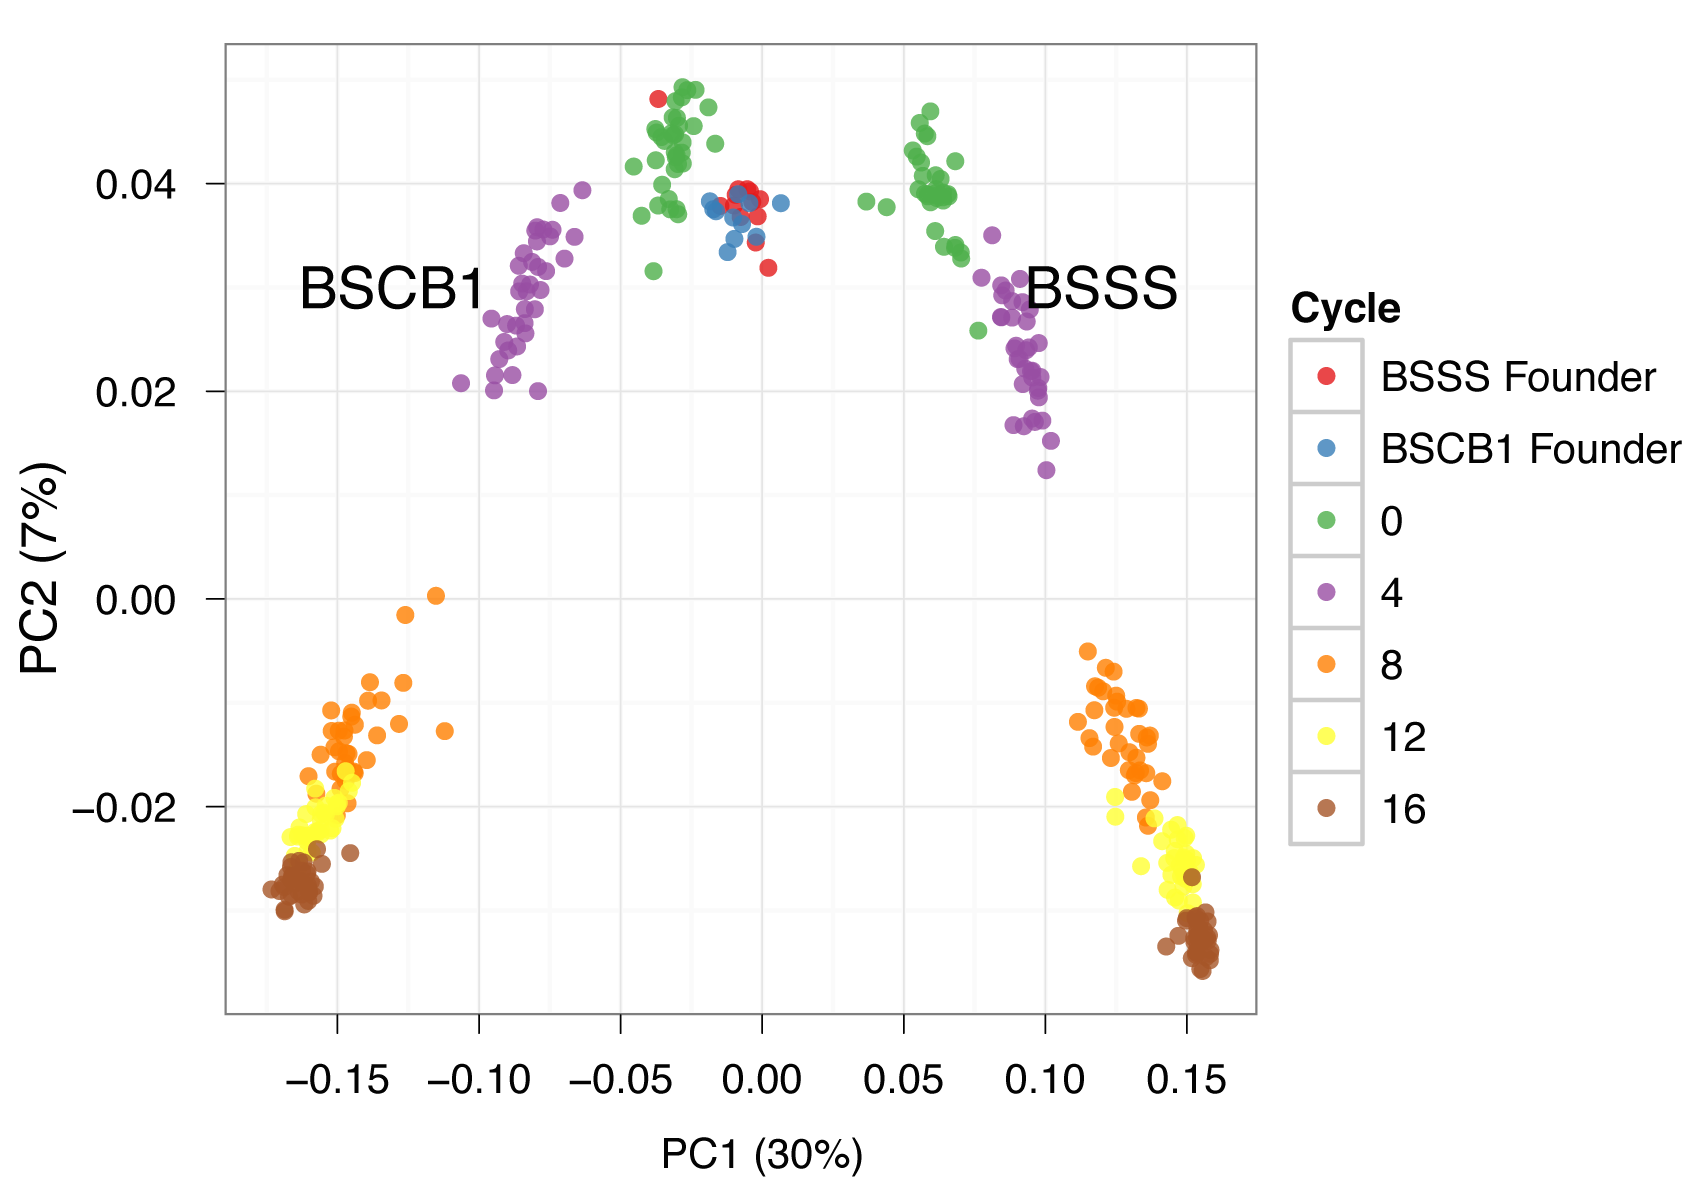
\includegraphics[width=0.5\textwidth]{fig1}
   \renewcommand{\baselinestretch}{0.9}
   \vspace{-3mm}
   \caption{Principal component analysis of the SNP data from Iowa RRS. The axes represent the first two eigenvectors from an analysis of cycles 0-16, with projection of the founder lines onto the vector space. The variation explained by each eigenvector is given in parentheses on the axes. The populations steadily diverge at increasing cycles, with less distinction visible between the founder groups. The comparatively large distance between cycles 4 and 8 corresponds to a switch from one to two generations of selfing at each cycle. The smaller separation between cycles 8-16 corresponds to an increase in effective population size from ten to twenty. The BSSS cycle 0 population has drifted away from the BSSS founders, despite the absence of intentional selection during the creation and maintenance of cycle 0.
} 
\vspace{-6mm}
    \label{fig:pca}
  \end{center}
\end{figure}
%%%%%%%%%%%%%%%%%%%%%%%%%%%%%%%%%%%%%%%%%% FIGURE

No new genetic material was intentionally introduced into either population after the experiment's inception, so the substantial increase in genetic distance could only arise from the loss of genetic diversity within each population. 
Consistent with previous studies of the Iowa RRS \citep{messmer1991genetic, labate1997molecular,  hagdorn2003molecular, hinze2005population}, genome-wide genetic diversity (expected heterozygosity, H) decreases steadily across cycles of selection in both populations (Figure \ref{fig:decline}). \jri{do all these citations make sense here? I just copied these from the abstract}
The loss of heterozygosity is smaller when the two populations are considered together, indicating the loss of different alleles within BSCB1 and BSSS. 
This genetic differentiation is reflected by the tenfold increase in $F_{ST}$ between the founder lines and the populations at cycle 16. 

%%%%%%%%%%%%%%%%%%%%%%%%%%%%%%%%%%%%%%%%%% FIGURE
\begin{figure}[tb]   
  \begin{center}
   \vspace{-0mm}
   \includegraphics[width=0.5\textwidth]{fig2}
   \renewcommand{\baselinestretch}{0.9}
   \vspace{-3mm}
   \caption{Heterozygosity \rev{(H, left panel) and $F_{ST}$ (right panel)} plotted as a function of selection cycle in each population. \rev{Heterozygosity is shown for each population separately and then for the total population pooling all plants.}
} 
\vspace{-6mm}
    \label{fig:decline}
  \end{center}
\end{figure}
%%%%%%%%%%%%%%%%%%%%%%%%%%%%%%%%%%%%%%%%%% FIGURE

We noticed an irregular increase in the number of polymorphic markers between BSSS cycles 4 and 8 (Table \ref{tab:s2}). 
All of these newly polymorphic markers were present at extremely low frequency and were spread among various individuals. 
This may represent a series of minor alleles that were not captured in our sample of cycle 4 individuals and thus appeared to ‘resurface’ at cycle 8. 
Alternatively, the pattern may be the result of minor contamination at some point in the population’s history. 
It was observed that an allele of the sugary gene associated with sweet corn appeared in the population at this time (O.S. Smith, personal communication), suggesting contamination may be the cause. 
However, the low frequency of the ‘new’ alleles (typically only one or two alleles out of 72 possible in 36 diploid samples) means their effect on population diversity is minimal.  
We did not attempt to incorporate this contamination into our simulation approaches, as it only makes our tests for low heterozygosity slightly more conservative.

\subsection*{Fixation of large genomic regions}
Figure \ref{fig:heterotic} shows heterozygosity varying along the genome at cycle 16 of each population. 
Of particular note are extremely large pericentromeric regions of zero or near-zero heterozygosity spanning tens of megabases. 
These regions experience low rates of meiotic recombination, which creates an expanded physical map relative to their genetic length \citep{ganal2011a-large}. 
In general, the majority of fixed haplotype segments are small ($<2$ cM) in genetic space regardless of their physical size; one exception is 7 cM region on chromosome 1 in the BSCB1 population. 

\begin{figure*}[tb]   
  \begin{center}
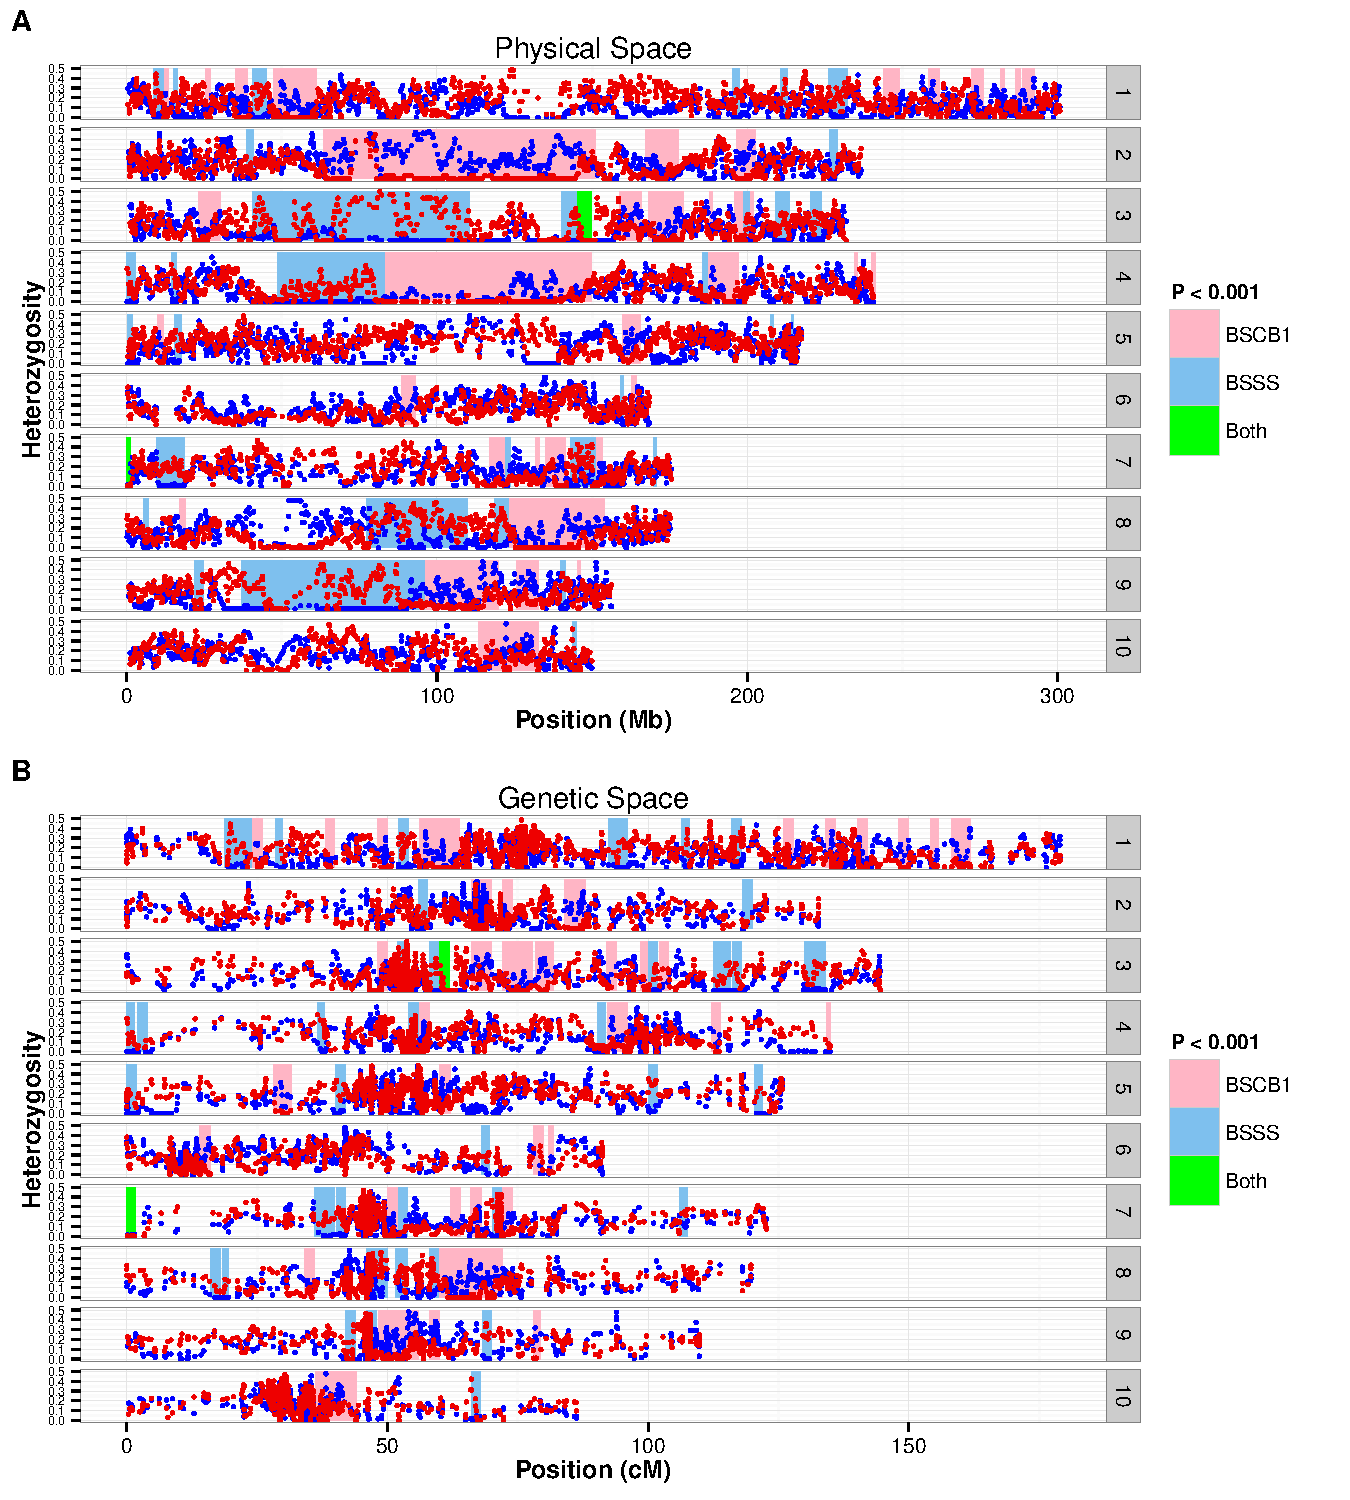
\includegraphics[width=0.7\linewidth]{fig_S2_combined}
   \caption{Heterozygosity at cycle 16 across all ten chromosomes in each population, calculated on 15-marker sliding windows with 5 marker steps. Heterozygosity values in BSSS (blue dots) and BSCB1 (red dots) are superimposed in one panel. 2 cM windows of heterozygosity lower than 10 of 10,000 simulations ($P<0.001$) are shaded in light blue (BSSS) or pink (BSCB1), \rev{and correspond to a genome-wide false discovery rate of $<3\%$ in both populations.} Two regions genome-wide show significantly low heterozygosity in both populations and are shaded green. (A) Physical map. (B) Genetic map. \rev{The same data are plotted separately for each population in Figure \ref{fig:s2}.}} 
    \label{fig:heterotic}
  \end{center}
\end{figure*}

The sheer physical size of the pericentromeric regions yields extremely high marker density on the genetic map, allowing for clear resolution of haplotype phasing and recombination breakpoints. 
To further examine the fixation in these regions, we computationally imputed haplotype phase in the BSSS and BSCB1 populations and used the phased data to track haplotype frequencies and founder of origin. 
In most cases, these fixed haplotypes can be traced back to single founder inbreds. 
For example, in BSSS, a 60 Mb (1.2 cM) region of chromosome 9 became fixed by cycle 12 and traces back to the founder Os420, and in BSCB1, a 60 Mb (0.7 cM) region became fixed on chromosome 4 and traces back to A340 (Figure \ref{fig:genphys}).
Table \ref{tab:fix} gives a summary of the large genomic regions that have become fixed or nearly fixed by cycle 16. 
These regions represent blocks of linked loci that show no evidence of recombination since at least the development of the founding inbred lines in the 1920’s and 1930’s.
	
%%%%%%%%%%%%%%%%%%%%%%%%%%%%%%%%%%%%%%%%%% FIGURE
\begin{figure*}[tb]   
  \begin{center}
  % \vspace{-0mm}
   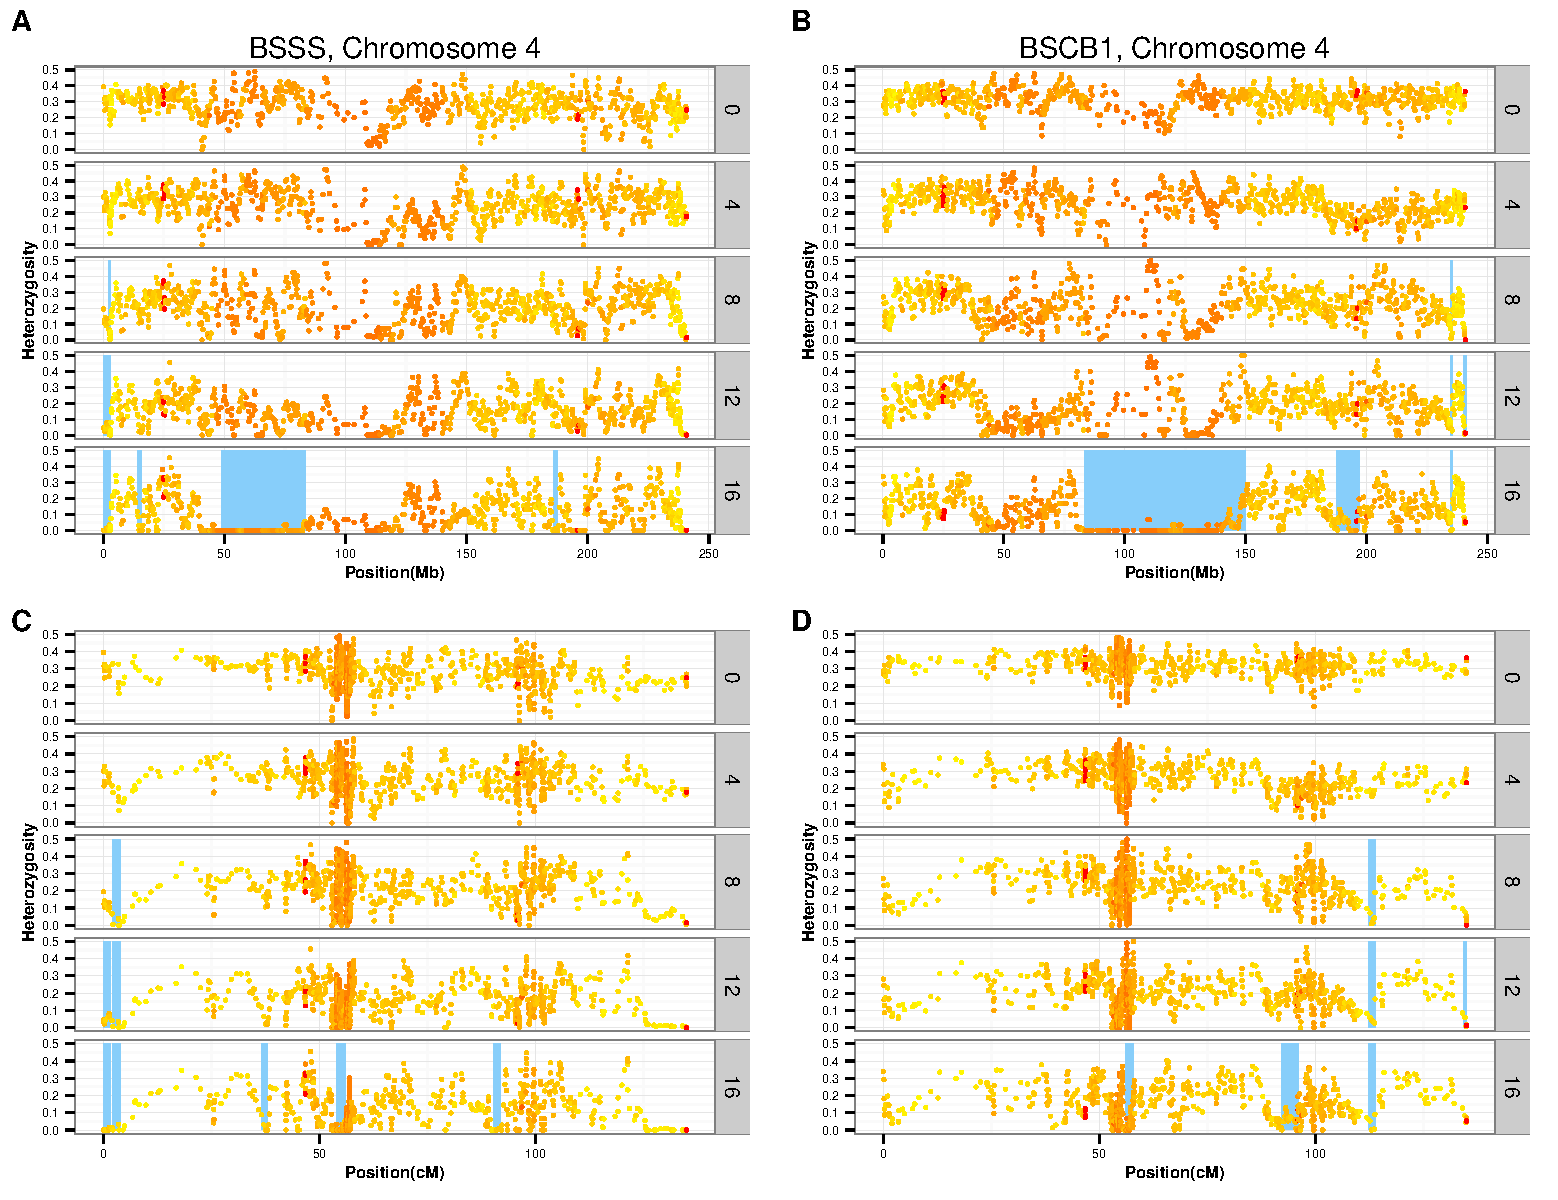
\includegraphics[width=0.8\linewidth]{Fig4/chrom4_combined}
 %  \renewcommand{\baselinestretch}{0.9}
 %  \vspace{-3mm}
   \caption{\rev{Heterozygosity} in each cycle across chromosome 4 of the BSSS (left) and  BSCB1 (right) plotted on the physical (top) and genetic (bottom) map. \rev{Each panel consists of five plots representing cycles 0,4,8,12, and 16 of the experiment. Heterozygosity} is calculated on 15-marker sliding windows, with 5 marker steps between each calculation. Each data point is color-coded based on a linear transformation of recombination rate (red = low recombination rate). Shaded regions represent 2 cM windows with heterozygosity values significantly lower than expected by simulation at a given cycle. \rev{Light and darker shading denotes significance at $P<0.0025$ and $P<0.001$, respectively. Plots for other chromosomes are shown in in Figure \ref{fig:others2}}. Comparing the physical and genetic maps reveals that the regions of fixation are extremely small genetically, but some contain much of the physical content of the chromosome.
} 
\vspace{-6mm}
    \label{fig:genphys}
  \end{center}
\end{figure*}
%%%%%%%%%%%%%%%%%%%%%%%%%%%%%%%%%%%%%%%%%% FIGURE	


\begin{table*}[t]
\caption{Ancestry of haplotypes fixed in the cycle 16 population.}
\fontsize{10}{12}\sf
\centering
   \begin{threeparttable}

\label{tab:fix}
\begin{tabular}{llllll}
Population &	 Chr.& Interval (cM) & Interval (Mb) &	Founder & Derived Lines \\
BSSS       & 3          & 53.6-55.3            & 67.7-123              & CI187-2        & B94                               \\
BSSS       & 3          & 57.3-64.8              & 129.2-157.1           & ND\tnote{\emph{a}}           & B89, B94                          \\
BSSS       & 4          & 52.8-55.6            & 39.9-82.7             & CI187-2        & B89, B94, B67, B72, B39, B43      \\
BSSS       & 9          & 41.1-44.8            & 20.8-26.6             & Oh7\tnote{\emph{b}}           & B89, B94, B43, B17, B72, B84, B67 \\
BSSS       & 9          & 45.7-47.5\tnote{\emph{c}}           & 30.8-90.4             & Os420          & B89, B94                          \\
BSCB1      & 2          & 67-67.5            & 80.6-114.5            & CC5            & B90, B91, B95, B97, B99           \\
BSCB1      & 4          & 55.6-57            & 82.7-140              & ND\tnote{\emph{a}}            & B90, B95, B97                     \\
BSCB1      & 8          & 61.5-67.7            & 125.1-145.6           & P8             & B90, B97, B91, B99, B54           \\\hline 
\end{tabular}
   \begin{tablenotes}
      \footnotesize
      \item[\emph{a}]{ND = Not Determined (Either a recombinant haplotype or originates from an un-genotyped founder)}
      \item[\emph{b}]{Although Oh7 is a BSCB1 founder, it is a descendant of CI.540, an un-genotyped BSSS founder. BSSS segments matching Oh7 presumably derive from CI.540}            
      \item[\emph{c}]{Founders Ind\_B2 (BSSS), CI187-2 (BSSS), R4 (BSCB1), and I205 (BSCB1) are all IBD at this region of chromosome 9}
   \end{tablenotes}
\end{threeparttable}
\end{table*}


\subsection*{The role of genetic drift}
There is clear evidence of phenotypic improvement in response to selection in the Iowa RRS populations (Smith, 1983; Keeratinijakal and Lamkey, 1993; Schnicker and Lamkey, 1993; Holthaus and Lamkey, 1995; Brekke et al., 2011a; Brekke et al., 2011b; Edwards, 2011) and large changes in genetic structure indicated by molecular markers. 
A central issue for these maize populations and others like them is whether the changes observed at the molecular level are caused directly by selection on phenotype, or indirectly due to the genetic drift that selection imposes through inbreeding and small effective population sizes. 
To gauge the roles of selection and drift, we conducted simulations of the crossing and selection schemes used in the RRS experiment.
Selection was executed at random in each simulation, so the patterns observed across simulations represent the expected distribution of effects caused only by recombination and genetic drift. 
We conducted 10,000 simulations, \rev{modeling recombination using the IBM genetic map \citep{lee2002expanding}, which is based on a cross between between a BSSS-derived inbred line used to construct the reference genome (B73) and an inbred with  with co-ancestry from both the BSSS and BSCB1 founder germplasm (Mo17).} 	

\begin{figure*}[tb]   
   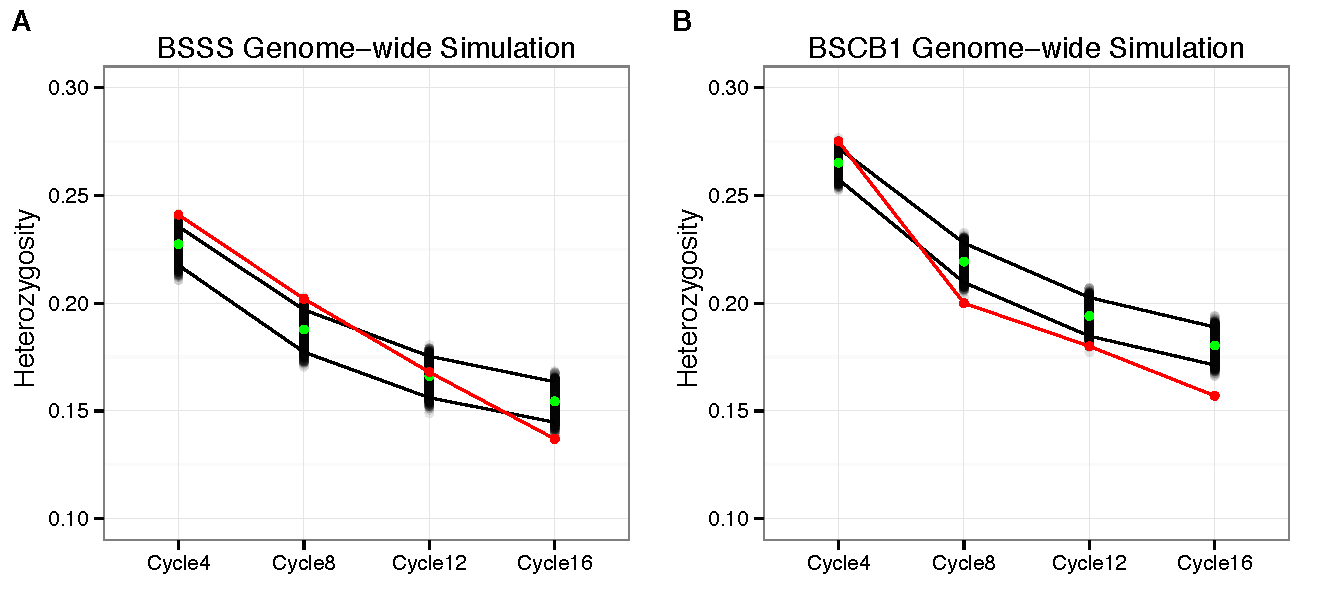
\includegraphics[width=0.7\linewidth]{Fig_S1_combined.pdf}
   \caption{Heterozygosity in each population, observed vs. simulated data. Heterozygosity was calculated as the average across all markers genome-wide  in the BSSS (A)  and BSCB1 (B) populations. The observed data is marked by the red line, the simulations by gray dots, and the median of the simulations by a green dot. \rev{Black lines represent the 95\% quantiles of the simulated data.} \jri{is that interpretation of the black lines correct?}} 
    \label{fig:compare_to_sims}
\end{figure*}

Averaged across the genome, the vast majority of the reduction in diversity observed in both populations can be attributed to genetic drift. 
Nonetheless, we do observe \rev{differences from values generated under our neutral simulations} (Figure \ref{fig:compare_to_sims}). 
The observed data show higher than expected heterozygosity at cycle 4, \rev{which could be explained by several factors, including differences between simulated and actual breeding practices, under-sampling of diversity in cycle 0, selection acting to increase the frequency of initially rare haplotypes, or even selection acting to maintain heterozygosity \citep[e.g.][]{McMullen2009,Gore2009a} } \jri{where is this excess of diversity? if it's all pericentromeric can we argue for the first hypothesis?}

As the cycles progress, heterozygosity falls more rapidly than expected in both populations, and the observed values at cycle 16 are significantly lower than the simulated data.  
Simulations across a number of different marker densities were consistent with this result (data not shown). 

To examine the behavior of specific regions, we compared observed and simulated results for each 2 cM segment of the genome. 
The dynamics observed across most of the genome are largely insensitive to window size (we tested from 2-4 cM, data not shown), and are consistent with strong genetic drift imposed by \rev{the experimental design}. 
A subset of loci were flagged as significant (Figure \ref{fig:heterotic}), and these loci almost always overlapped regions of fixation or near-zero heterozygosity in one population. 
\rev{Simulated values in these regions are often quite low as well (Supplementary File S2), however, indicating that drift alone can explain most of the drop in diversity.}

Since the population size of the Iowa RRS is small (10-20), many biallelic SNPs should fix by chance regardless of their starting minor allele frequencies. 
\rev{Observed differences from the simulated neutral expectation} thus do not arise from changes in allele frequencies per se, but rather from the fixation of linked markers across larger than expected genetic distances. 
The validity of significance cutoffs therefore depend on the accuracy of our genetic map.
While the maize genetic map is known to vary among genetic backgrounds across short distances \citep{McMullen2009}, broad-scale patterns of recombination appear relatively stable across diverse germplasm \citep[][but see \citet{bauer2013intraspecific}]{rodgers2015recombination}.
\rev{Differences between} observed and simulated results could be due to selection, variation or inaccuracy in the genetic map, or a combination of these factors. 

To explore the roles of selection and drift independent of the genetic map, we returned to the large regions of fixation in the centromeres which showed no recombination across the full RRS experiment. 
Given the lack of recombination, each of these regions can be analyzed by the simulation of a single locus, and the high density of markers allows the clear resolution of the individual haplotypes. 
We used the computationally phased data to measure the frequency of the fixed haplotype at each cycle, and assessed the probability of observing the fixation event given the initial frequency. 
The BSSS chromosome 9 haplotype fixed at cycle 16 was at low frequency at cycle 0 (7 out of 68 haplotypes), but increased rapidly in frequency by cycle 8 (66 out of 70 haplotypes). 
Simulation of the haplotype as a single locus in the RRS experiment produces this increase in frequency in only 3.9\% of 1000 independent simulations, whereas the haplotype was lost in over 80\% of the simulations. 
In BSCB1, a 30 Mb, 1.6 cM region of chromosome 2 became nearly fixed by cycle 8 (67/70) despite a prevalence of 4/72 at cycle 0, which occurred 1.5\% of the time by simulation. 
Although these results suggest that selection may have pushed these haplotypes to fixation, the fact that fixation of such a rare haplotype still occurred in some simulations speaks to the strong genetic drift imposed upon the BSSS and BSCB1 populations.   
Interestingly, each of these two genomic regions harbored a different cycle 0 haplotype at higher frequency, but these higher-frequency haplotypes were subsequently lost within the RRS population. 
In other cases, the haplotypes which eventually fixed were at moderate frequency in the cycle 0 populations and drift to fixation in the majority of simulations.

\section*{Discussion}
\jri{need to mention that the complementation we are seeing is not large effect deleterious that were likely purged during early inbreeding but instead many weakly deleterious things. need to add Drosophila and other cites. need to add Sprague 1983. then need to shorten/tighten up.} 
 
Our analysis of diversity in the Iowa RRS experiment reveals a steady loss of diversity in the BSSS and BSCB1 populations as they became increasingly differentiated from one another over time.
Principal component analysis shows that as the effective population size and the rates of inbreeding were altered, the rates of change in population structure were altered as well. 
These patterns of population structure, diversity, and differentiation between BSSS and BSCB1 can be largely reproduced by simulation without any selection, supporting the hypothesis that the majority of the genetic structure observed can be attributed to genetic drift alone, despite effective selection for phenotypic improvement. 
This drift was driven by inbreeding through self-pollination and the small effective population sizes used to select a limited number of high-performing, potentially related individuals at each cycle.  

\rev{The trends observed in the Iowa RRS are reflected in similar recurrent selection experiments \citep{romay2012effect,lamkey2014relative}.
Reciprocal recurrent selection serves as a model for the method of hybrid maize improvement \citep{duvick2004long}, and similar patterns of diversity and population structure can be seen broadly across North American maize germplasm \citep{van2012historical}. 
Given the lack of strong selection signals in each case, genetic drift has most likely played a large role in the current genetic structure of modern maize. }	
	
Several key inbreds in the ‘stiff-stalk’ heterotic group, B73, B37 and B14, were derived from the BSSS population \citep{darrah1986, troyer1999background}. 
B37 and B14 were derived from cycle 0, and B73 was derived from a half-sib recurrent selection program also started with the BSSS population. 
We examined these three inbreds at the pericentromeric regions listed in Table \ref{tab:fix} \jri{correct?}, and found that in most cases they carry different haplotypes from those that rose to high frequency in the RRS experiment.  
Near isogenic lines that substitute these centromeric haplotypes from key inbreds could be used to determine if the haplotypes at high frequency in cycle 16 of BSSS provide a phenotypic advantage when crossed with BSCB1. 

Both our study and previous work \citep{labate1997molecular} identified genetic differentiation between cycle 0 of BSSS and the founder inbreds, \rev{likely reflecting the loss of some rare alleles.
If this differentiation reflects drift during population maintenance before initiation of the RRS, it may have impacted the trajectory of the RRS program and of key inbreds derived from BSSS. 
However, cycle 0 has also undergone maintenance since the beginning of the RRS experiment, so some} drift may have occurred during this time as well.
	
Although drift can explain most of the genetic structure genome-wide, phenotypic data provide clear evidence that selection has altered the frequencies of favorable alleles in the BSSS and BSCB1 populations. 
Numerous experiments have shown that the selected populations and the hybrids formed from them are superior to their cycle 0 ancestors \citep{smith1983evaluation, keeratinijakal1993responses, schnicker1993interpopulation, holthaus1995population}. 
Improvement occurred not only for hybrid yield, but concurrently for plant architecture and tolerance to high-density planting in both hybrids and inbreds \citep{brekke2011selection, brekke2011selectionb, edwards2011changes, lauer2012morphological}. 
Since these same trends are observed across wider North American germplasm \citep{tollenaar1989genetic}, identification and characterization of the loci conferring phenotypic improvement in BSSS and BSCB1 could reveal some of the genetic mechanisms by which maize yield has steadily improved over the decades. 
We find that the genomic regions of extremely low diversity evident at cycle 16 are unlikely to be produced by simulation, and heterozygosity falls more than expected across the genome as a whole.  
However, simulated and observed values are often close, so overall the signature of selection is difficult to detect at any given locus. 
This is due in large part to a limitation of statistical power imposed by inbreeding and low effective population sizes.
\citet{lorenz2015selection} analyze a similar selection experiment with comparable effective population size and also find little little statistical evidence for selection on individual loci in spite of genetic gain for the trait of interest.
Nonetheless, we show that an identity-by-descent, haplotype based approach provides additional power, as it can distinguish between the fixation of rare and common haplotypes. 
However, the results of single locus simulations are sensitive to sampling error and drift caused by population maintenance. 
In this case, it is difficult to assess significance with only a single population to test. This type of analysis is more effective across several replicated populations, which can control for genetic drift due to the independence between the selections in each replicate \citep{lamkey2014relative}. 
	
\citet{van2012historical} assessed variation in and tested for selection across a wider range of North American maize germplasm using the same SNP array. 
Although selected loci were identified in that study, the overall effects on genomic diversity and haplotype patterns were relatively small compared with the impact of domestication. 
That study was a wide survey across many germplasm sources. 
The limited overall impact of selection could arise because different haplotypes and loci are selected in different breeding programs. 
In support of this idea, we find that the most likely targets of selection between the BSSS and BSCB1 populations occur at non-overlapping loci. 
This non-overlap between putatively selected loci in complementary populations has also been observed in commercial breeding programs \citep{feng2006temporal}.

\subsection*{Heterosis}

The observation that the same targets of selection are not observed in the opposing heterotic populations bears implications for the genetic mechanisms responsible for heterosis and the success of maize hybrids. 
Classic overdominance models of heterosis predict that at a single locus, two distinct alleles confer heterozygote advantage when combined, while the dominance model predicts that heterosis is driven by dominance effects and the complementation of linked alleles in low-recombination regions (dominance or pseudo-overdominance). 
In the case of true overdominance, we selection should lead to decreased heterozygosity at a locus in both populations as complementary haplotypes are fixed in each group \rev{\citep[e.g.][]{guo2014maize}}.
We find \rev{little evidence to support this genetic phenomenon, finding only two 2 cM windows genome-wide in which both populations show significantly reduced heterozygosity.} 
The observed pattern instead favors a dominance model, where fixation of a haplotype in one population simply selects against that same haplotype in the other population. 
Because most deleterious alleles are rare in both heterotic groups \citep{Mezmouk2014}, most haplotypes in the second population will have a different suite of deleterious variants and will complement the fixed haplotype reasonably well, such that selection will have little impact on diversity in the second population. 
Our data are consistent with such a process having been important for hybrid improvement in the Iowa RSS experiment, and the lack of extreme differentiation seen over time across US Corn Belt germplasm is consistent with a role for such selection in maize hybrid improvement in general \citep{van2012historical}.

Our results are consistent with the dominance and pseudo-overdominance models, but we caution that the exact outcome of particular models will depend strongly on the effects of selection, drift, and the frequencies of beneficial alleles. 
Disentangling these factors remains a major challenge that will require careful simulation of maize breeding using a wider range of parameters. 
This is especially true because in a model of hybrid complementation, genetic drift in one population can alter the selective value of alleles in the other population. 
When drift and selection interact in such a manner, tests for selection that attempt to independently partition the effects of each force may not provide the full picture. Furthermore, uncertainties in the fine-scale relationship between genetic and physical distance make it difficult to assign significance in forward-simulation approaches. 
In the end, the best test for selection of specific genomic regions will ultimately be conducted by phenotypic observation in the field in balanced tests of different haplotypes. 
In the case of individual breeding programs, genome-wide genotyping such as we conducted here can identify the lines carrying the recombinant haplotypes and introgressions necessary to conduct such an experiment. 

\begin{acknowledgments}
We thank Oscar ``Howie'' Smith and members of the Ross-Ibarra lab for comments on earlier versions of the manuscript. J.P.G received support for this research as a Merck Fellow of the Life Sciences Research Foundation. This research was supported by the National Science Foundation (IOS-0820619) and funds provided to USDA-ARS (MDM). Names of products are necessary to report factually on available data: however, neither the USDA, nor any other participating institution guarantees or warrants the standard of the product and the use of the name does not imply approval of the product to the exclusion of others that may also be suitable.
\end{acknowledgments}

\bibliography{references.bib}
\bibliographystyle{geneticsT2}

\suppl
\renewcommand{\thefigure}{S\arabic{figure}}
\renewcommand{\thetable}{S\arabic{table}}

%%%%%%%%%%%%%%%%%%%%%%%%%%%%%%%%%%%%%%%%%% FIGURE
\begin{figure*}   
  \begin{center}
   \vspace{-0mm}
   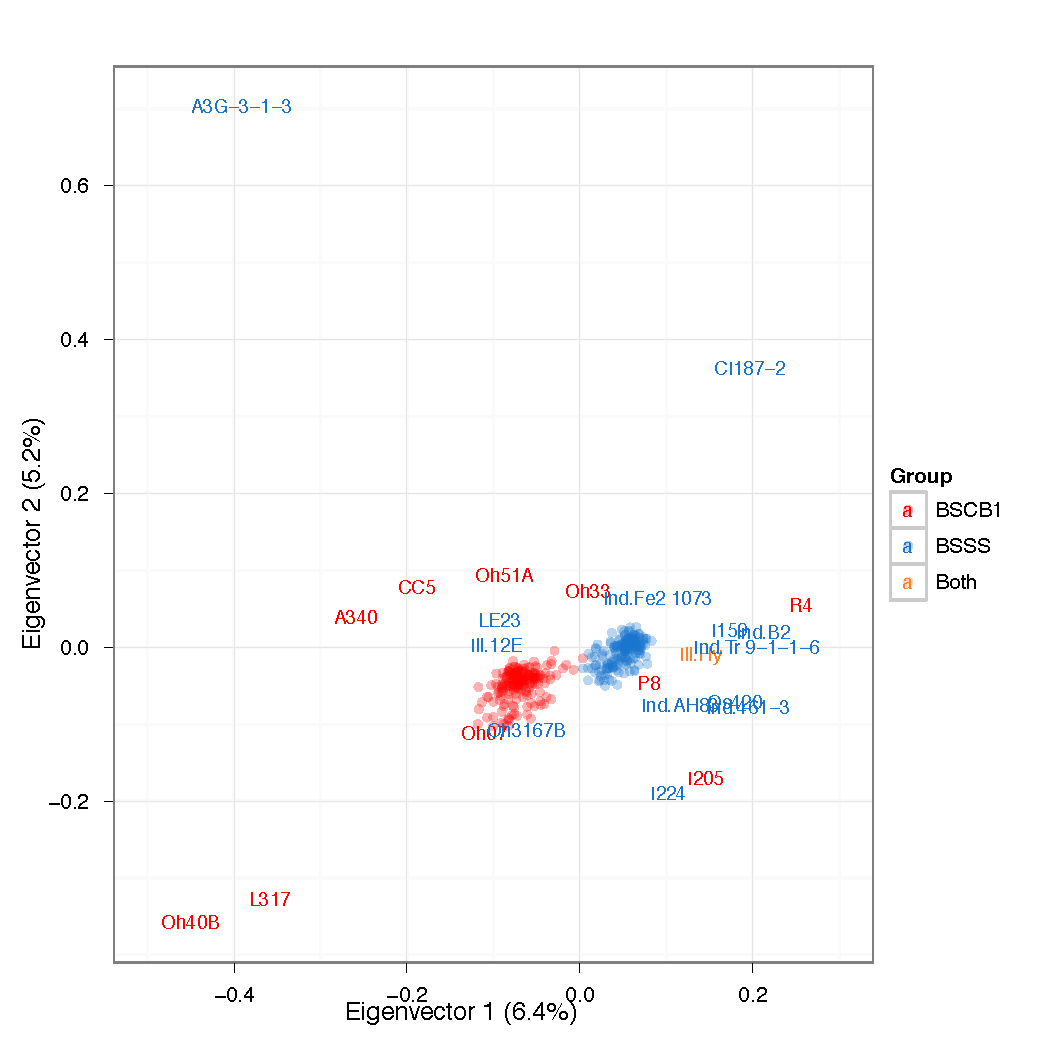
\includegraphics[width=0.7\linewidth]{pca_founders}
   %\renewcommand{\baselinestretch}{0.9}
   \vspace{-3mm}
   \caption{ Principle component analysis of founder inbred lines. The names of founder inbreds are shown on the graph; all other points represent BSSS (blue) and BSCB1 (red) individuals projected onto the PCA of the founders.
} 
\vspace{-6mm}
    \label{fig:sfounders}
  \end{center}
\end{figure*}
%%%%%%%%%%%%%%%%%%%%%%%%%%%%%%%%%%%%%%%%%% FIGURE


%%%%%%%%%%%%%%%%%%%%%%%%%%%%%%%%%%%%%%%%%% FIGURE
\begin{figure*}   
  \begin{center}
   \vspace{-0mm}
   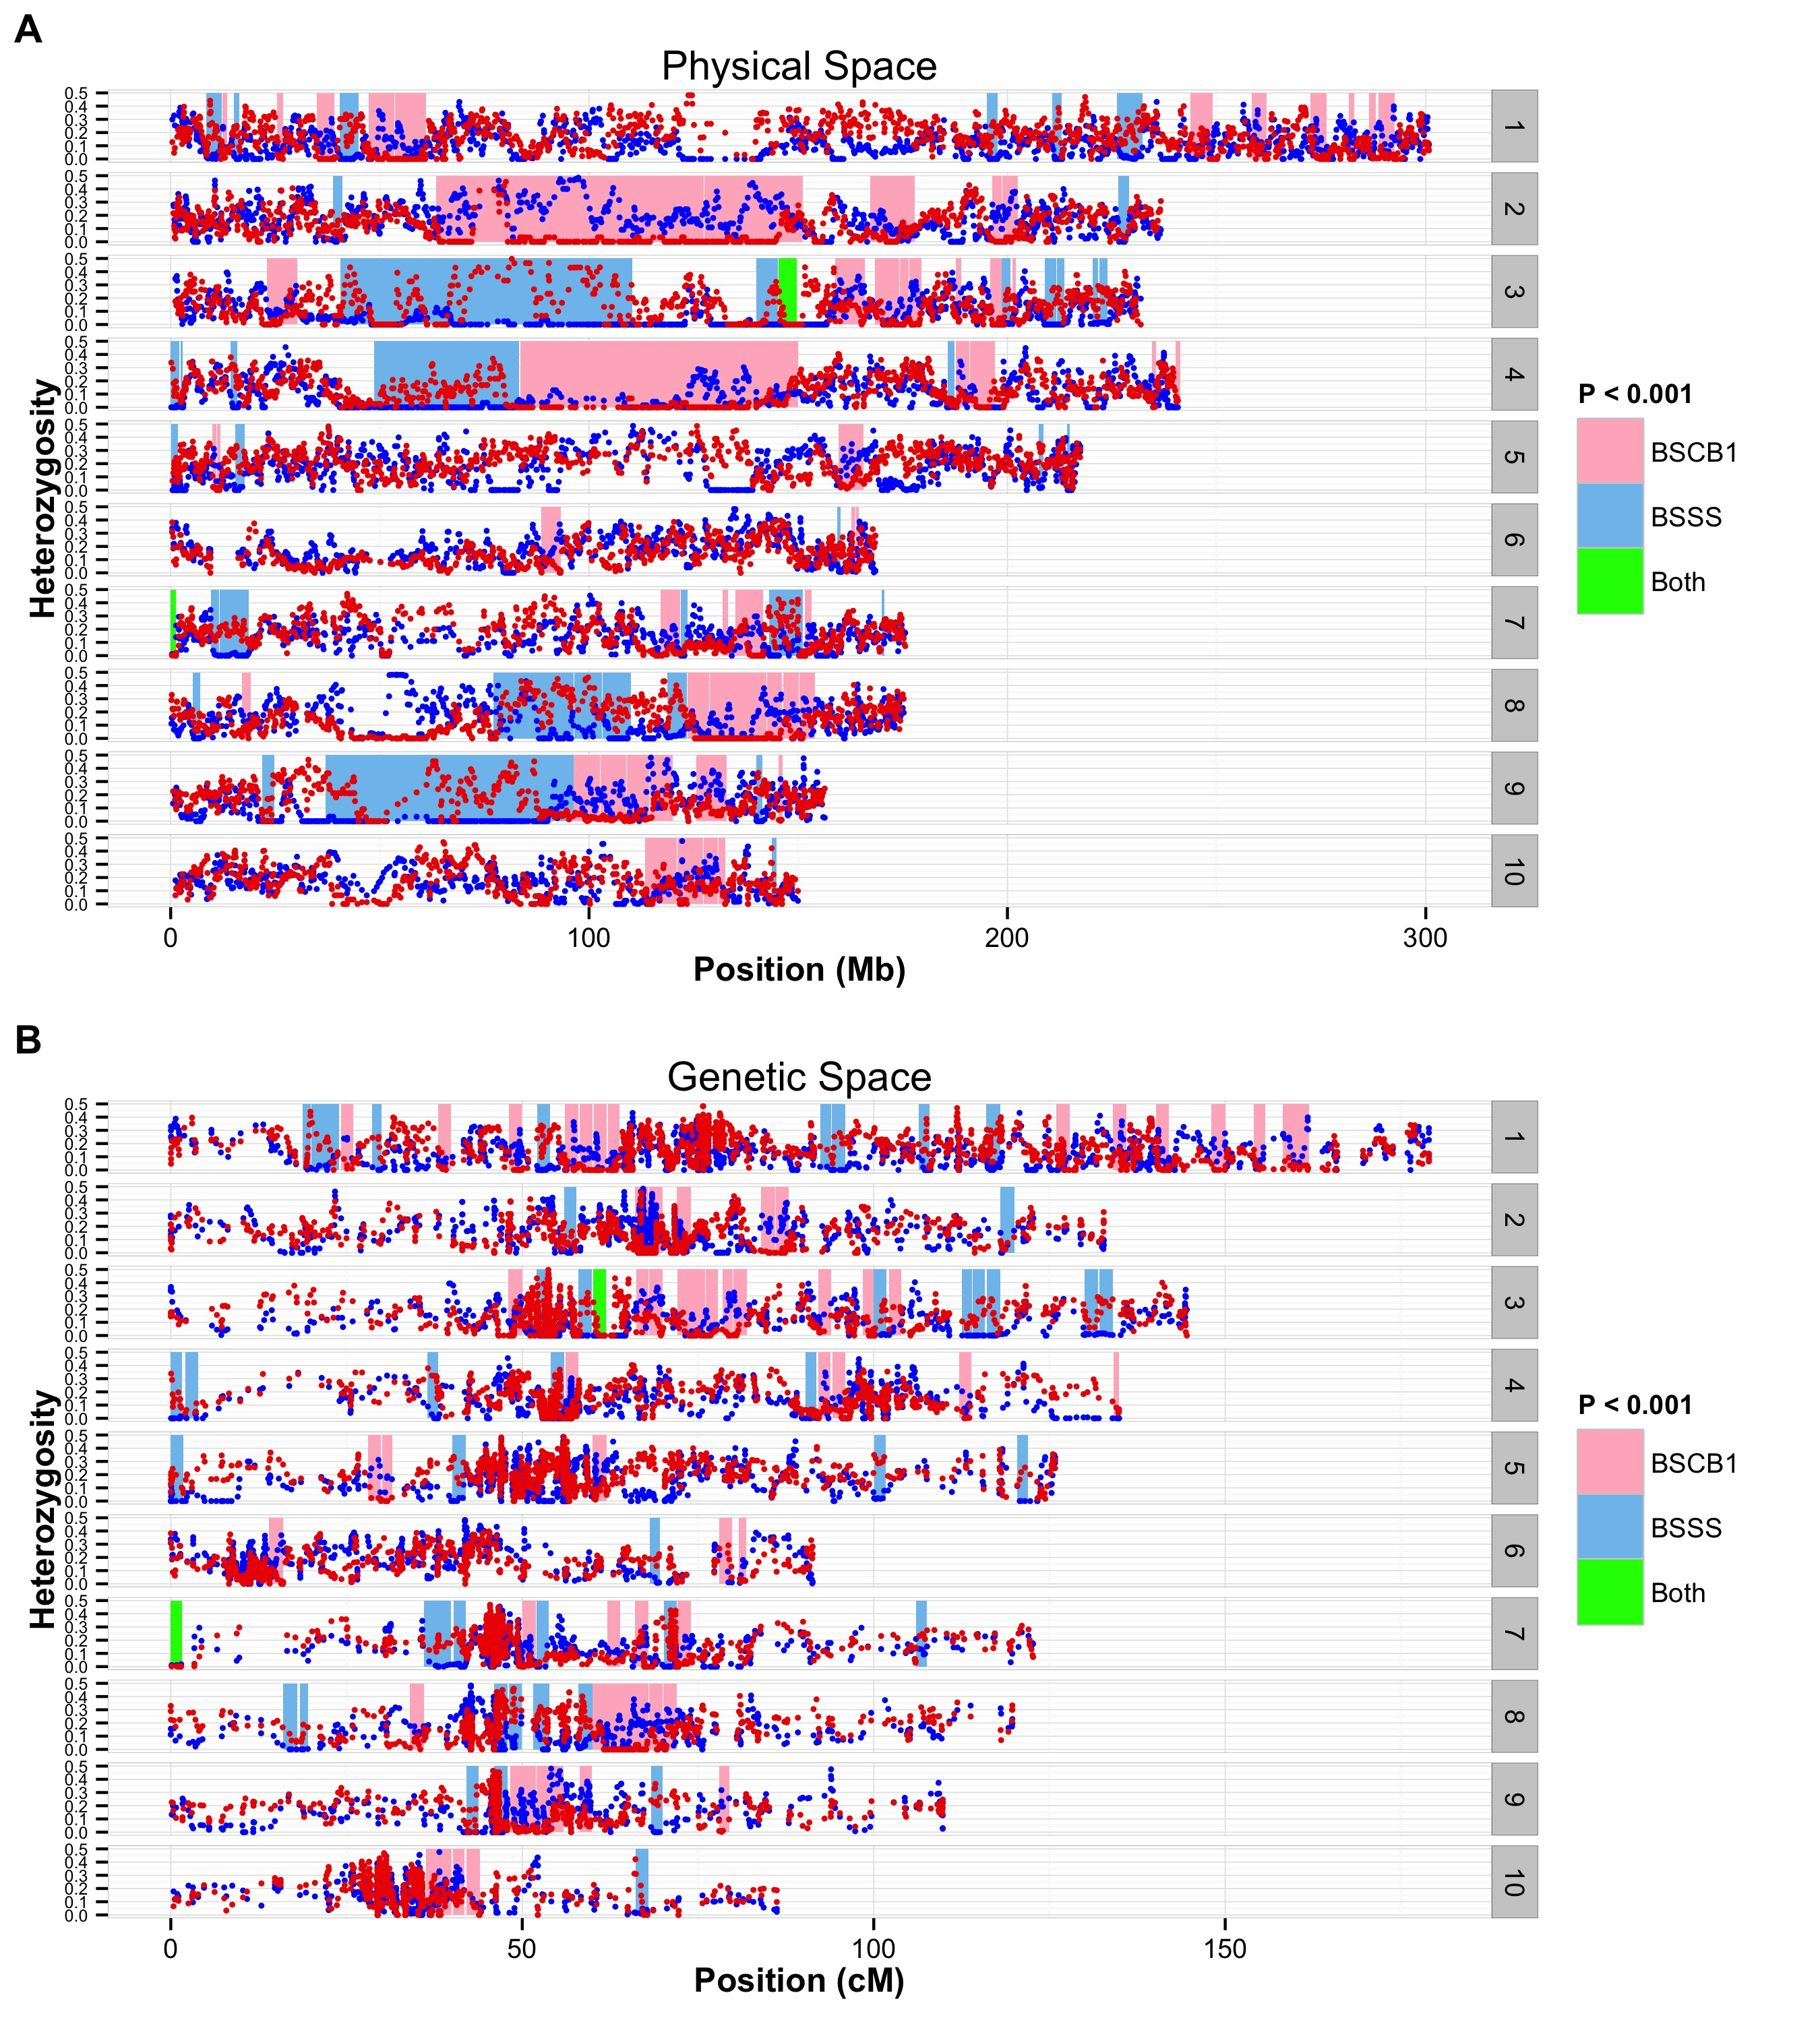
\includegraphics[width=0.7\linewidth]{fig3}
   %\renewcommand{\baselinestretch}{0.9}
   \vspace{-3mm}
   \caption{ Heterozygosity ($H$) at cycle16 across all ten chromosomes in each population.  $H$ is calculated on 15-marker sliding windows with 5 marker steps. Each point is plotted at the midpoint of the 15-marker window. 
} 
\vspace{-6mm}
    \label{fig:s2}
  \end{center}
\end{figure*}
%%%%%%%%%%%%%%%%%%%%%%%%%%%%%%%%%%%%%%%%%% FIGURE

%%%%%%%%%%%%%%%%%%%%%%%%%%%%%%%%%%%%%%%%%% FIGURE
\begin{center}
\Image[width=0.7\linewidth]{Fig4/chrom1_combined}{} \\
\Image[width=0.7\linewidth]{Fig4/chrom2_combined}{} 
\newpage
\Image[width=0.7\linewidth]{Fig4/chrom3_combined}{} \\
\Image[width=0.7\linewidth]{Fig4/chrom5_combined}{} 
\newpage
\Image[width=0.7\linewidth]{Fig4/chrom6_combined}{} \\
\Image[width=0.7\linewidth]{Fig4/chrom7_combined}{} 
\newpage
\Image[width=0.7\linewidth]{Fig4/chrom8_combined}{} \\
\Image[width=0.7\linewidth]{Fig4/chrom9_combined}{} 
\newpage
\Image[width=0.7\linewidth]{Fig4/chrom10_combined}{}  
\captionof{figure}{Heterozygosity in each cycle across chromosomes of the BSSS (left) and BSCB1 (right) plotted on the physical (top) and genetic (bottom) map. Details are as in Fig. 4.}
    \label{fig:others2}
\end{center}




%\begin{figure*}   
%  \begin{center}
%   \vspace{-0mm}
%   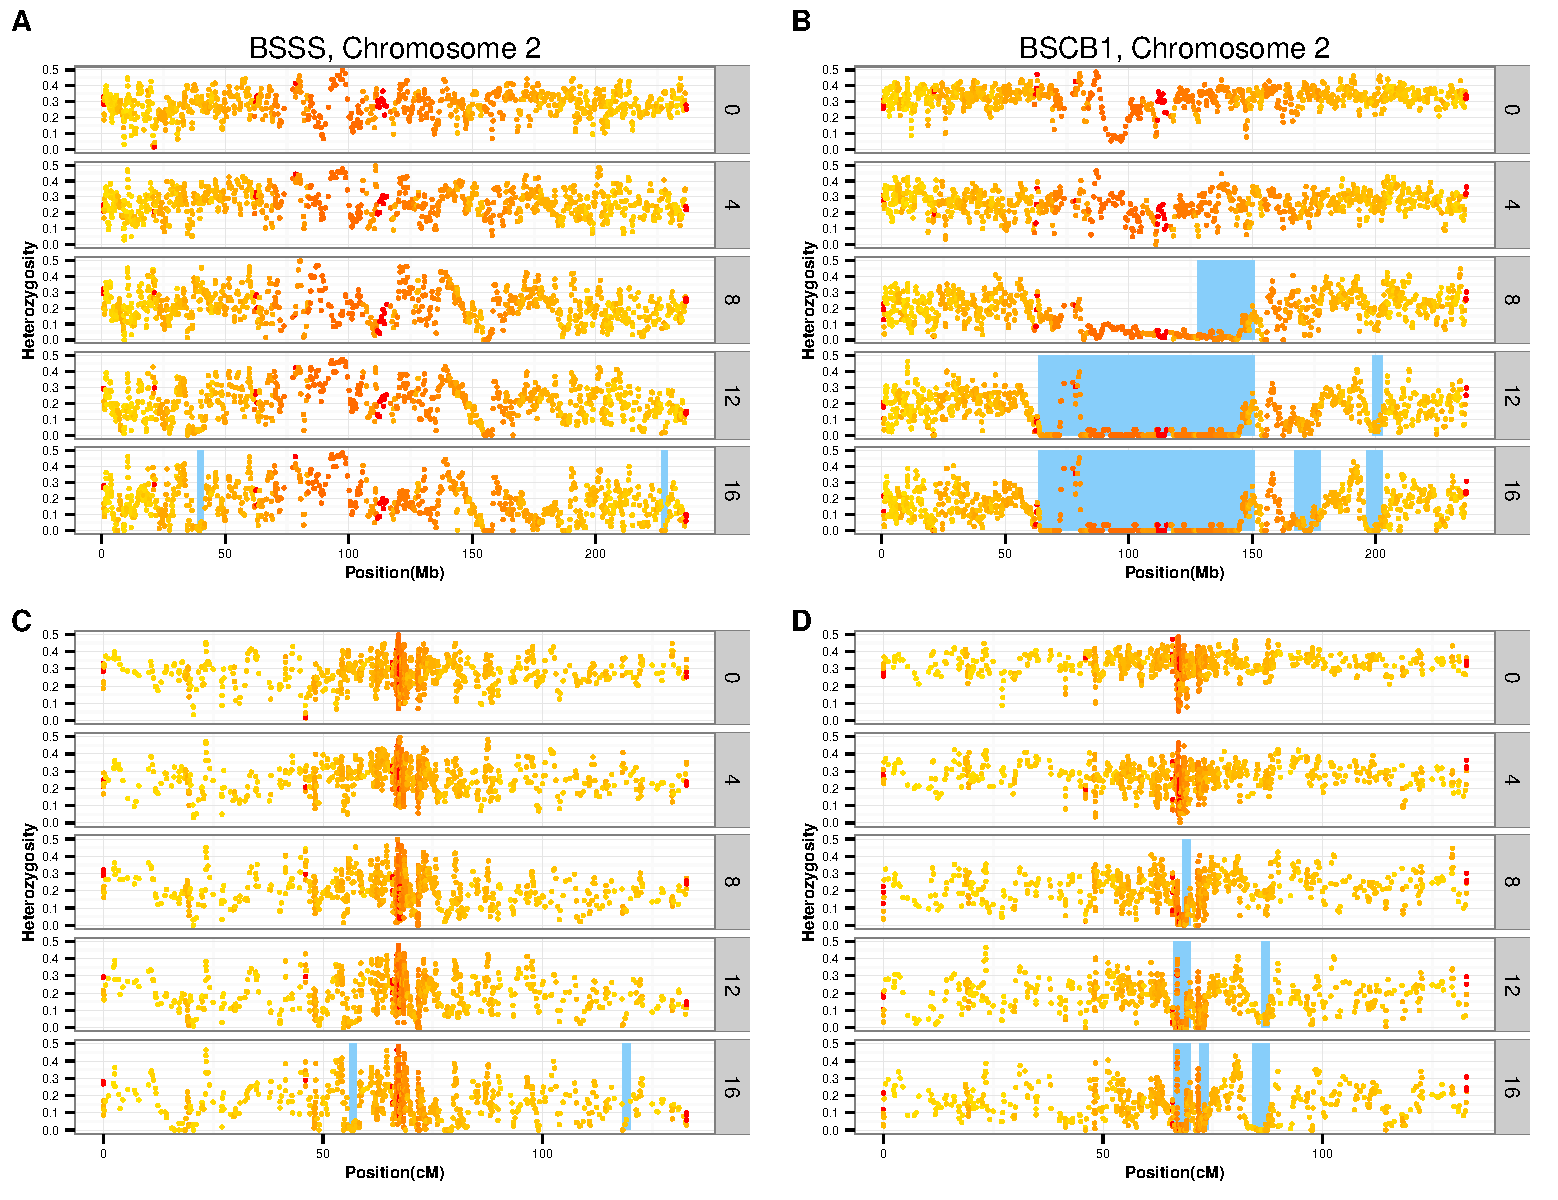
\includegraphics[width=0.7\linewidth]{Fig4/chrom2_combined.pdf}
%   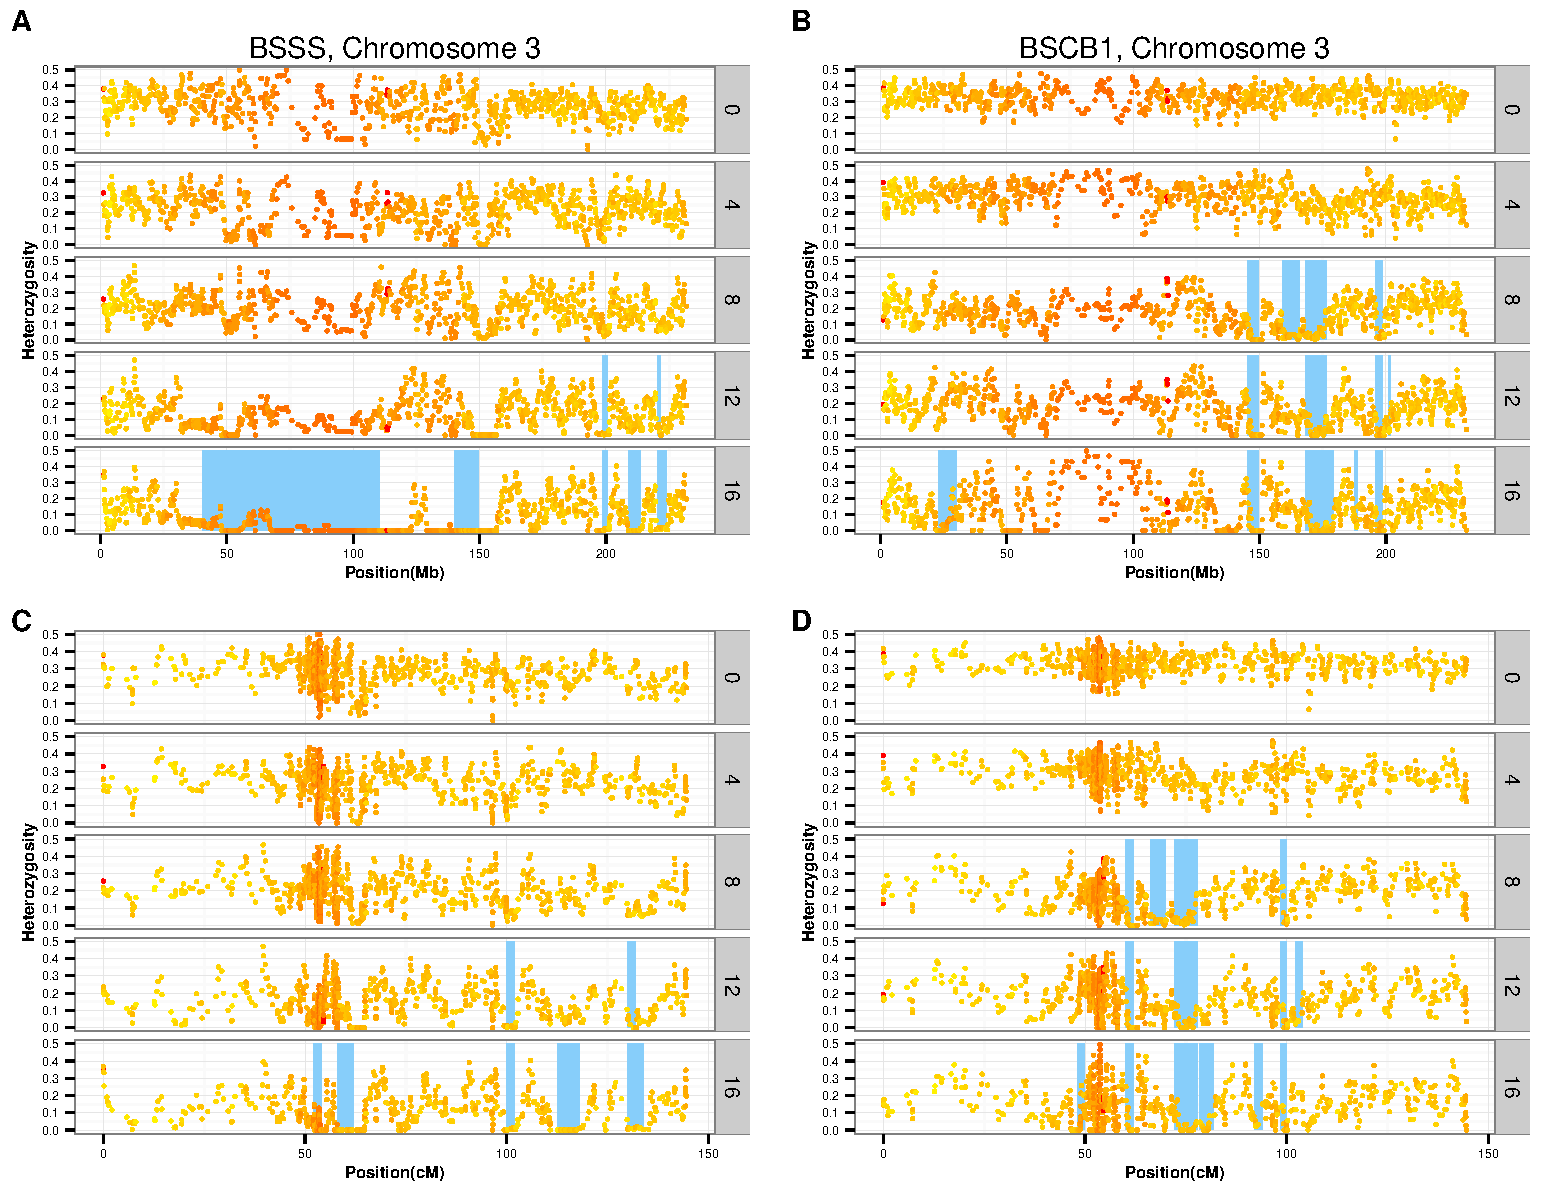
\includegraphics[width=0.7\linewidth]{Fig4/chrom3_combined.pdf}
%   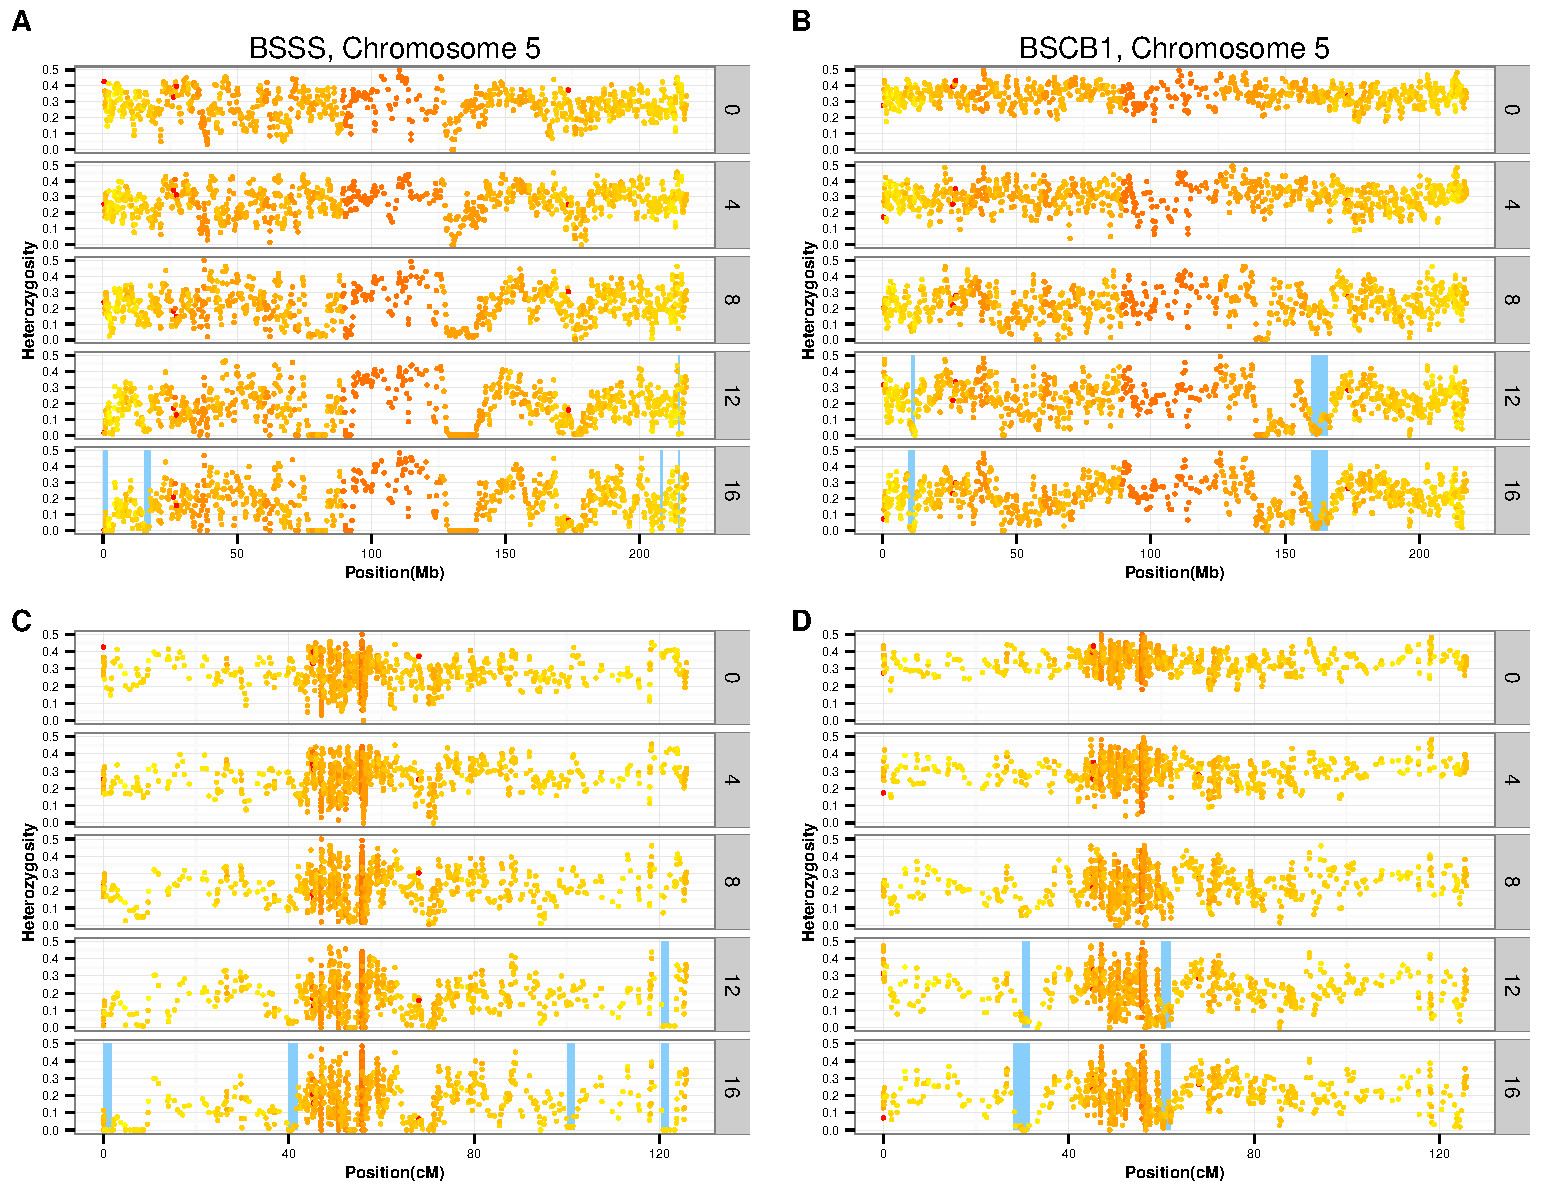
\includegraphics[width=0.7\linewidth]{Fig4/chrom5_combined.pdf}
%   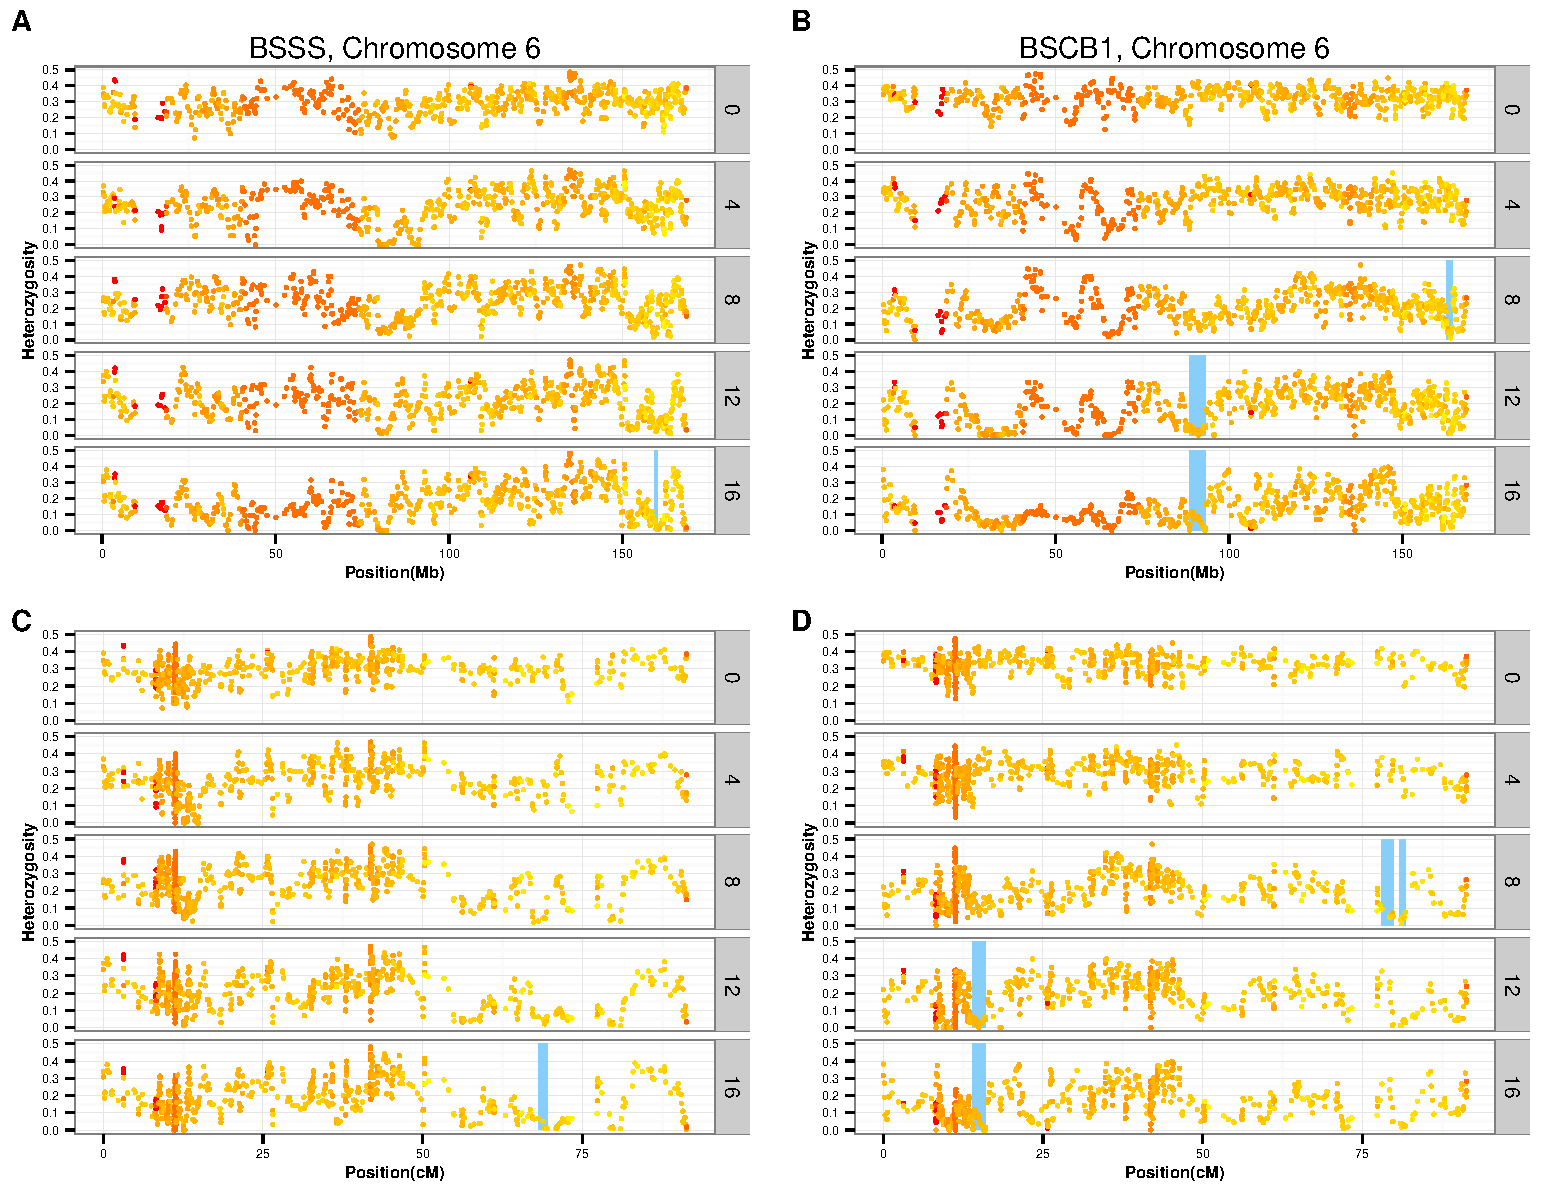
\includegraphics[width=0.7\linewidth]{Fig4/chrom6_combined.pdf}
%   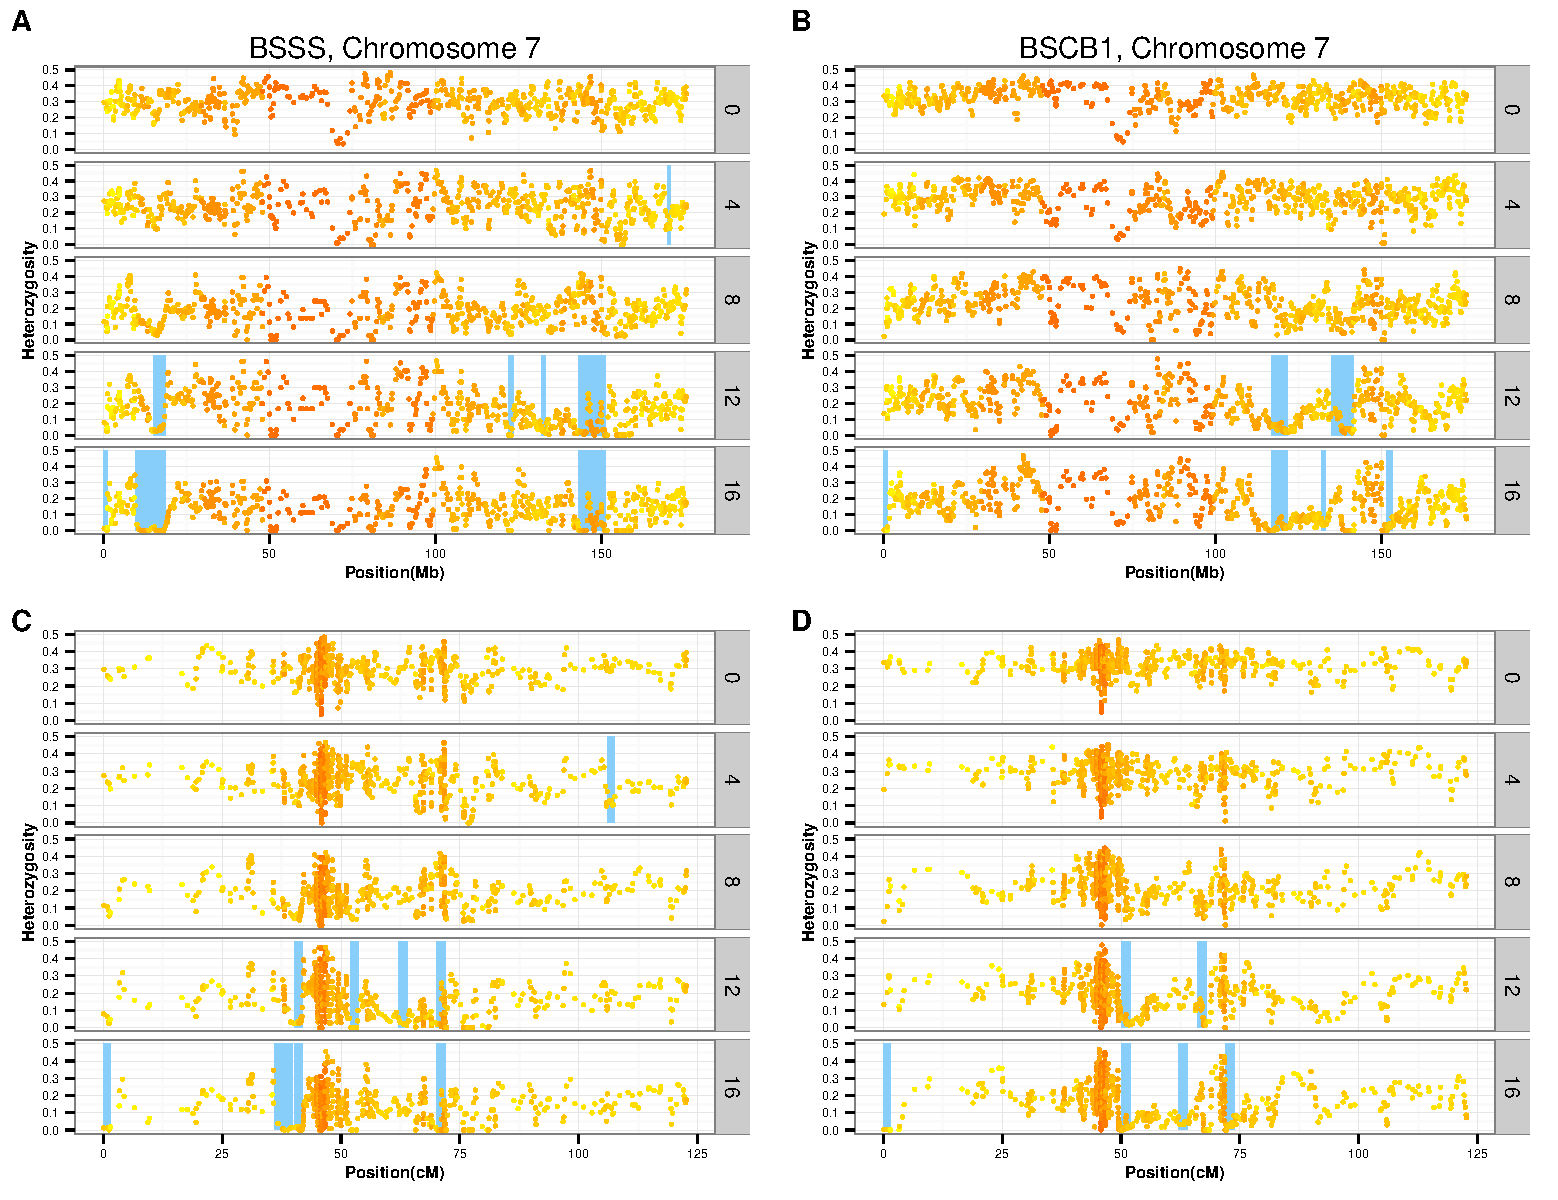
\includegraphics[width=0.7\linewidth]{Fig4/chrom7_combined.pdf}
%   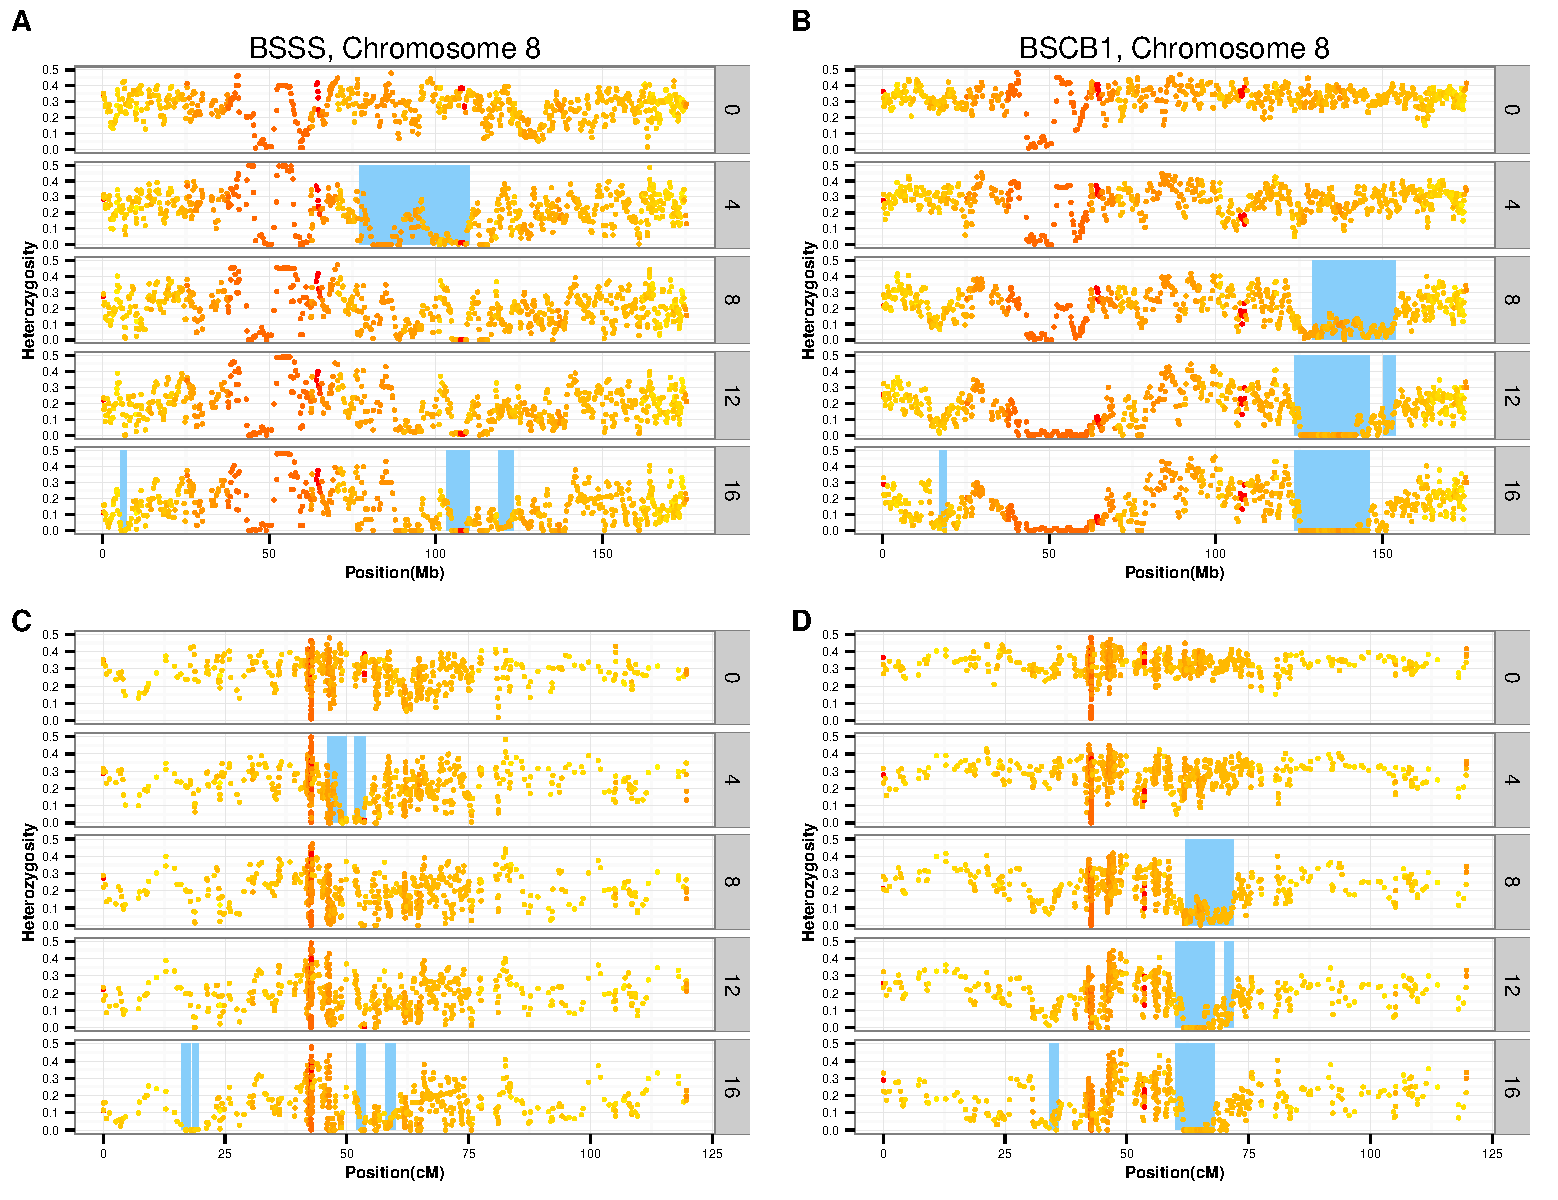
\includegraphics[width=0.7\linewidth]{Fig4/chrom8_combined.pdf}
%   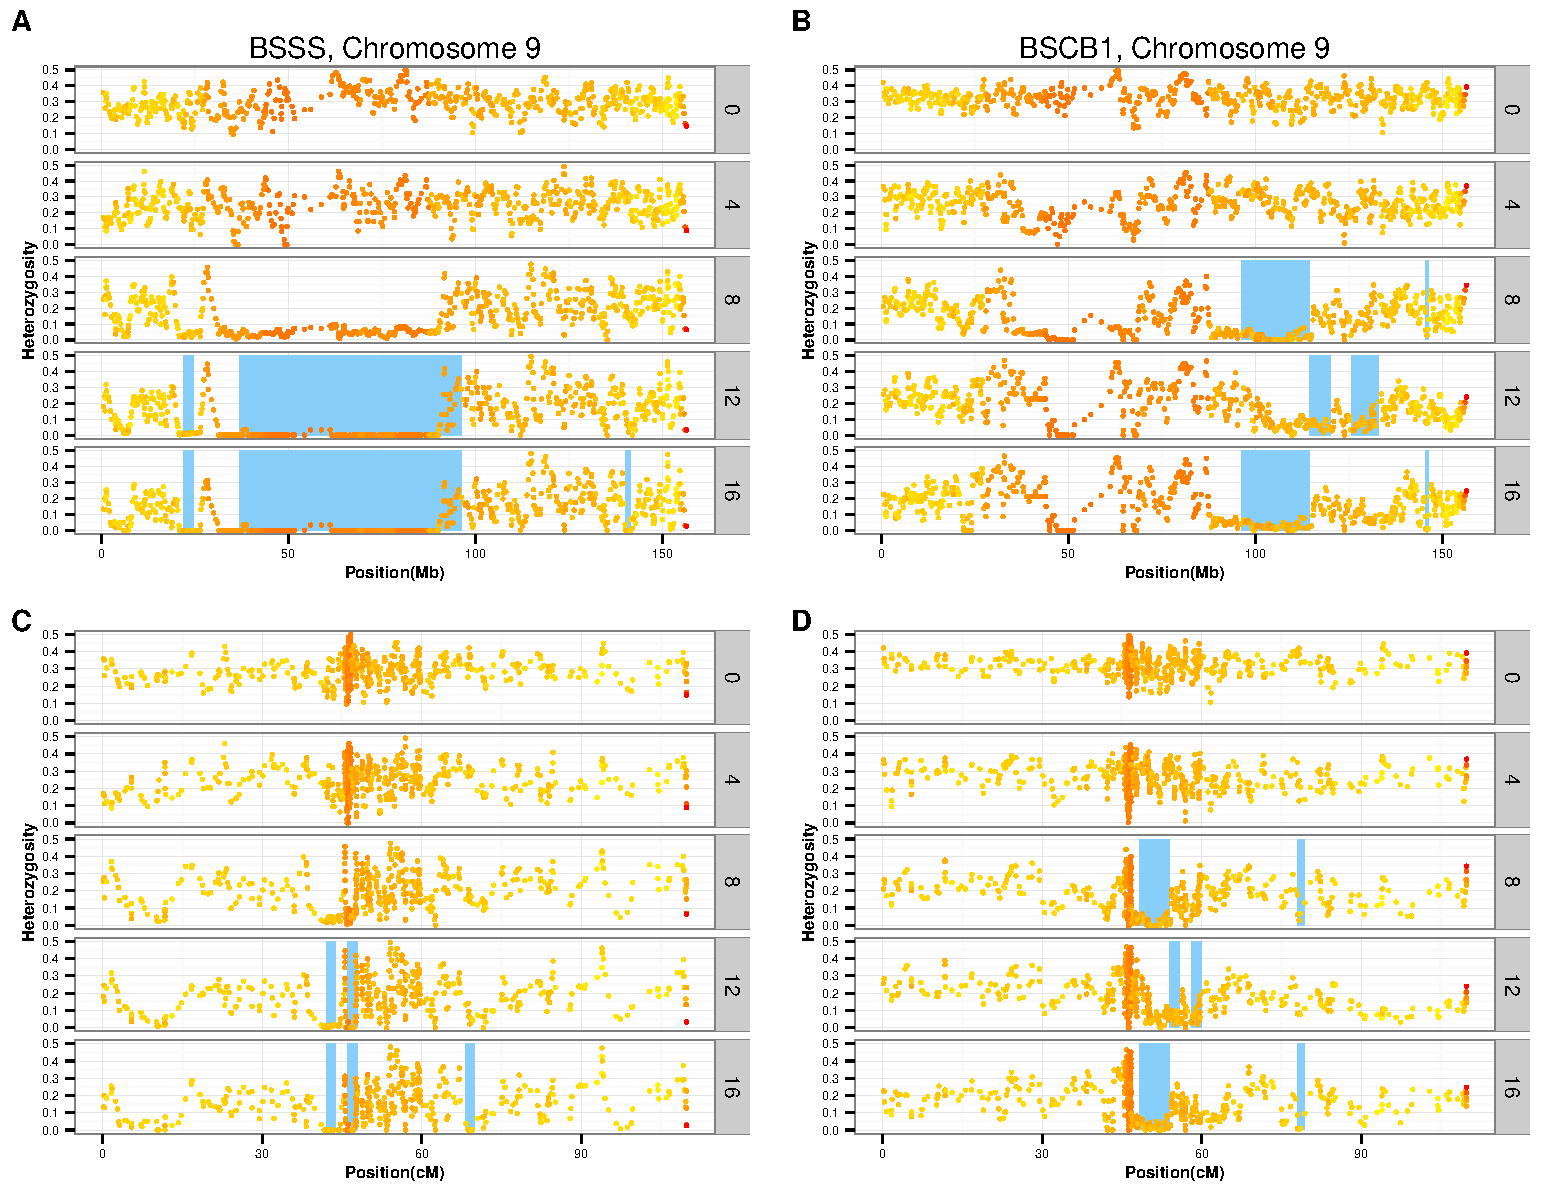
\includegraphics[width=0.7\linewidth]{Fig4/chrom9_combined.pdf}
%   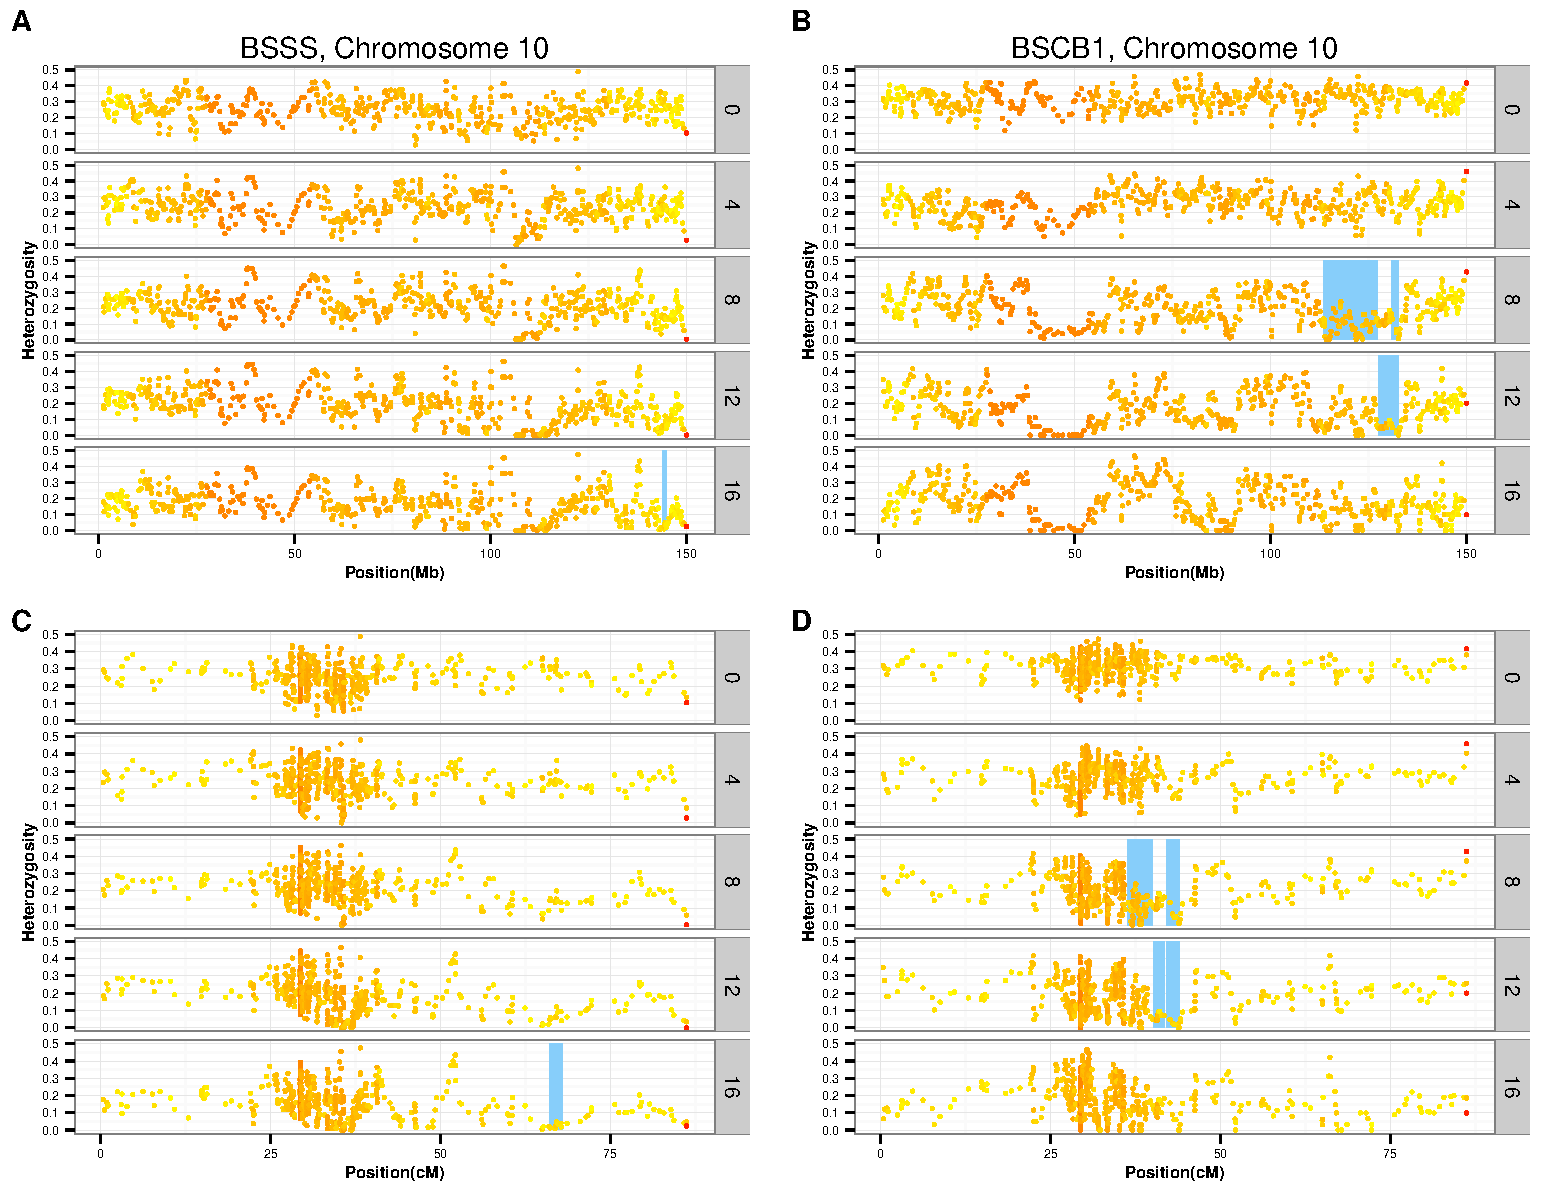
\includegraphics[width=0.7\linewidth]{Fig4/chrom10_combined.pdf}
%   %\renewcommand{\baselinestretch}{0.9}
%   \vspace{-3mm}
%   \caption{ Heterozygosity in each cycle across chromosomes of the BSSS (left) and BSCB1 (right) plotted on the physical (top) and genetic (bottom) map. Details are as in Fig. 4.
%} 
%\vspace{-6mm}
%    \label{fig:s2}
%  \end{center}
%\end{figure*}
%%%%%%%%%%%%%%%%%%%%%%%%%%%%%%%%%%%%%%%%%% FIGURE

\newpage

\begin{table}
\caption{Plants and Lines Genotyped in this study.
Backgrounds of the founder inbreds are from \citet{hagdorn2003molecular}}
\begin{tabular}{ | l | l | l | l | }

	{\bf Plants from the selection cycles} &  &  &  \\ 
	Population  & Cycle & \# plants &   \\ 
	BSSS & 0 & 34 &  \\ 
	BSSS & 4 & 36 &  \\ 
	BSSS & 8 & 35 &  \\ 
	BSSS & 12 & 36 &  \\ 
	BSSS & 16 & 36 &  \\ 
	BSCB1 & 0 & 36 &  \\ 
	BSCB1 & 4 & 36 &  \\ 
	BSCB1 & 8 & 35 &  \\ 
	BSCB1 & 12 & 36 &  \\ 
	BSCB1 & 16 & 36 &  \\ 
	 &  &  &  \\ 
	BSSS Founders Genotyped &  &  &  \\ 
	Inbred & Background / Pedigree &  &  \\ 
	Ind\_Tr9\_1\_1\_6 & Reid Early Dent (Troyer Strain) &  &  \\ 
	Oh3167B & Echelberger Clarage &  &  \\ 
	I224 & Iodent &  &  \\ 
	Ind467(744) & Reid Medium &  &  \\ 
	CI.187-2 & Krug-Nebraska Reid x IA Gold Mine &  &  \\ 
	Os420 & Osterland Yellow Dent &  &  \\ 
	I159 & Iodent &  &  \\ 
	A3G-3-1-3 & BL345BxIAI129 &  &  \\ 
	Ind\_Fe2\_1073* & Troyer Reid (Early) &  &  \\ 
	Ill\_Hy & IL High Yield &  &  \\ 
	Ill\_12E & unknown &  &  \\ 
	Ind\_AH83 & Funk 176A &  &  \\ 
	Ind\_B2* & Troyer Reid (Late Butler), parent of a founder &  &  \\ 
	LE23 & IL Low Ear &  &  \\ 
	*Parents of unavailable line F1B1 &  &  &  \\ 
	 &  &  &  \\ 
	BSCB1 Founders Genotyped &  &  &  \\ 
	Inbred & Background / Pedigree &  &  \\ 
	I205 & Iodent &  &  \\ 
	Oh51A & [(OH56xWf9)Oh56] (Wooster Clarage x ?) &  &  \\ 
	A340 & 4-29 x 64 (Silver King x Northwestern Dent) &  &  \\ 
	Ill\_Hy & IL High Yield &  &  \\ 
	Oh33 & Clarage &  &  \\ 
	Oh07 & C.I.540xIII.L &  &  \\ 
	R4 & Funk Yellow Dent &  &  \\ 
	Oh40B & eight line LSC composite &  &  \\ 
	P8 & Palin Reid &  &  \\ 
	L317 & LSC &  &  \\ 
	CC5 & Golden Glow (W23) &  &  \\ 
	 &  &  &  \\ 
	Founders not analyzed &  &  &  \\ 
	Inbred & Group & Reason &  \\ 
	CI.540 & BSSS & heterozygous genotype &  \\ 
	F1B1 & BSSS & unavailable &  \\ 
	CI.617 & BSSS & unavailable &  \\ 
	WD456 & BSSS & unavailable &  \\ 
	K230 & BSCB1 & source segregates phenotypically &  \\ 
	 &  &  &  \\ 
	Derived Lines Used &  &  &  \\ 
	Inbred & Group & Cycle & Notes \\ 
	B10 & BSSS & 0 & thrown out; poor data quality \\ 
	B42 & BSCB1 & 0 &  \\ 
	B14A & BSSS & 0 & Cuzco x B14 \\ 
	B43 & BSSS & 0 &  \\ 
	B10 & BSSS & 0 &  \\ 
	B37 & BSSS & 0 &  \\ 
	B44 & BSSS & 0 &  \\ 
	B17 & BSSS & 0 &  \\ 
	B69 & BSSS & 0 &  \\ 
	B39 & BSSS & 0 &  \\ 
	B90 & BSCB1 & 7 &  \\ 
	B40 & BSSS & 0 &  \\ 
	B54 & BSCB1 & 0 &  \\ 
	B78 & BSSS & 8 & from half-sib recurrent selection program \\ 
	B72 & BSSS & 3 & from half-sib recurrent selection program \\ 
	B84 & BSSS & 7 & from half-sib recurrent selection program \\ 
	B94 & BSSS & 8 &  \\ 
	B99 & BSCB1 & 10 &  \\ 
	B11 & BSSS & 0 &  \\ 
	B89 & BSSS & 7 &  \\ 
	B95 & BSCB1 & 7 &  \\ 
	B91 & BSCB1 & 8 &  \\ 
	B67 & BSSS & 0 &  \\ 
	B73 & BSSS & 5 & from half-sib recurrent selection program \\ 
	B97 & BSCB1 & 9 &  \\ 
	    \label{tab:s1}  % caption is needed to make this work
\end{tabular}
\end{table}
\newpage

\begin{table}
\caption{Evidence of minor contamination between cycles 4 and 8 in BSSS.}
\begin{tabular}{ | l | l | l | l | }
\hline
	\textbf{SNPs polymorphic in cycle} & \textbf{But not cycle} & \textbf{BSSS} & \textbf{BSCB1} \\ \hline
	4 & 0 & 290 & 225 \\ \hline
	8 & 0 & 2242 & 319 \\ \hline
	12 & 0 & 1227 & 181 \\ \hline
	16 & 0 & 344 & 128 \\ \hline
	8 & 4 & 4499 & 1081 \\ \hline
	12 & 4 & 2328 & 669 \\ \hline
	16 & 4 & 551 & 477 \\ \hline
	12 & 8 & 1821 & 1405 \\ \hline
	16 & 8 & 178 & 997 \\ \hline
	16 & 12 & 542 & 666 \\ \hline
	0 & Founders & 1202 & 1707 \\ \hline
	4 & Founders & 822 & 885 \\ \hline
	8 & Founders & 1201 & 798 \\ \hline
	12 & Founders & 816 & 550 \\ \hline
	16 & Founders & 445 & 460 \\ \hline
\end{tabular}
		    \label{tab:s2}  % caption is needed to make this work
\end{table}
\newpage

\begin{table}
\caption{Heterozygosity of SNPs in cycle 8 but not cycle 4 of the BSSS. }
\begin{tabular}{  l | l | l | }
\multicolumn{1}{l}{} & \multicolumn{1}{l}{BSSS} & \multicolumn{1}{l}{BSSS}   \\ \cline{2-3}
	Mean & 0.052 & 0.052   \\ \cline{2-3}
	Median & 0.028 & 0.028   \\ \cline{2-3}
\end{tabular}
\end{table}
\jri{are  numbers in table supposed to be the same? I checked the Pages doc and they are the same there too.}
\jpg{yeah, it means one or two instances of the allele in a pop of 36.} 


\begin{table}
\caption{Switch error rates from computationally phasing ‘hybrids’ simulated from derived inbred lines.}
\begin{tabular}{ | l | l | l | l | l | l | }

\hline
	\textbf{Simulated 'Hybrid'} & \textbf{Derived Lines Used as Priors} & \textbf{Population} & \textbf{Possible Switches} & \textbf{Switch errors} & \textbf{Rate} \\ \hline
	B11xB67 & all & BSSS & 12195 & 41 & 0.003 \\ \hline
	B17xB44 & all & BSSS & 12230 & 58 & 0.005 \\ \hline
	B39xB37 & all & BSSS & 11485 & 129 & 0.011 \\ \hline
	B43xB69 & all & BSSS & 12266 & 26 & 0.002 \\ \hline
	B73xB72 & all & BSSS & 12043 & 47 & 0.004 \\ \hline
	B78xB94 & all & BSSS & 11658 & 51 & 0.004 \\ \hline
	B89xB84 & all & BSSS & 11517 & 53 & 0.005 \\ \hline
	B11xB67 & cycle 0 & BSSS & 12195 & 45 & 0.004 \\ \hline
	B17xB44 & cycle 0 & BSSS & 12230 & 54 & 0.004 \\ \hline
	B39xB37 & cycle 0 & BSSS & 11485 & 126 & 0.011 \\ \hline
	BB43xB69 & cycle 0 & BSSS & 12266 & 32 & 0.003 \\ \hline
	B42xB54 & all & BSCB1 & 11260 & 38 & 0.003 \\ \hline
	B90xB97 & all & BSCB1 & 6499 & 52 & 0.008 \\ \hline
	B91xB95 & all & BSCB1 & 7830 & 56 & 0.007 \\ \hline
	B99xB97 & all & BSCB1 & 6779 & 52 & 0.008 \\ \hline
	BB42xB54 & cycle 0 & BSCB1 & 11260 & 57 & 0.005 \\\hline
\end{tabular}
	\label{tab:s3}  % caption is needed to make this work
\end{table} 

\end{document}

